%%%%%%%%%%%%%%%%%%%%%%%%%%%%%%%%%%%%%%%%%
% Lachaise Assignment
% LaTeX Template
% Version 1.0 (26/6/2018)
%
% This template originates from:
% http://www.LaTeXTemplates.com
%
% Authors:
% Marion Lachaise & François Févotte
% Vel (vel@LaTeXTemplates.com)
%
% License:
% CC BY-NC-SA 3.0 (http://creativecommons.org/licenses/by-nc-sa/3.0/)
% 
%%%%%%%%%%%%%%%%%%%%%%%%%%%%%%%%%%%%%%%%%

%----------------------------------------------------------------------------------------
%	PACKAGES AND OTHER DOCUMENT CONFIGURATIONS
%----------------------------------------------------------------------------------------

\documentclass{article}

%%%%%%%%%%%%%%%%%%%%%%%%%%%%%%%%%%%%%%%%%
% Lachaise Assignment
% Structure Specification File
% Version 1.0 (26/6/2018)
%
% This template originates from:
% http://www.LaTeXTemplates.com
%
% Authors:
% Marion Lachaise & François Févotte
% Vel (vel@LaTeXTemplates.com)
%
% License:
% CC BY-NC-SA 3.0 (http://creativecommons.org/licenses/by-nc-sa/3.0/)
% 
%%%%%%%%%%%%%%%%%%%%%%%%%%%%%%%%%%%%%%%%%

%----------------------------------------------------------------------------------------
%	PACKAGES AND OTHER DOCUMENT CONFIGURATIONS
%----------------------------------------------------------------------------------------

\usepackage{amsmath,amsfonts,stmaryrd,amssymb} % Math packages

\usepackage{enumerate} % Custom item numbers for enumerations

\usepackage[ruled]{algorithm2e} % Algorithms

\usepackage[framemethod=tikz]{mdframed} % Allows defining custom boxed/framed environments

\usepackage{listings} % File listings, with syntax highlighting
\lstset{
	basicstyle=\ttfamily, % Typeset listings in monospace font
}

%----------------------------------------------------------------------------------------
%	DOCUMENT MARGINS
%----------------------------------------------------------------------------------------

\usepackage{geometry} % Required for adjusting page dimensions and margins

\geometry{
	paper=a4paper, % Paper size, change to letterpaper for US letter size
	top=2.5cm, % Top margin
	bottom=3cm, % Bottom margin
	left=2.5cm, % Left margin
	right=2.5cm, % Right margin
	headheight=14pt, % Header height
	footskip=1.5cm, % Space from the bottom margin to the baseline of the footer
	headsep=1.2cm, % Space from the top margin to the baseline of the header
	%showframe, % Uncomment to show how the type block is set on the page
}

%----------------------------------------------------------------------------------------
%	FONTS
%----------------------------------------------------------------------------------------

\usepackage[utf8]{inputenc} % Required for inputting international characters
\usepackage[T1]{fontenc} % Output font encoding for international characters

\usepackage{XCharter} % Use the XCharter fonts

%----------------------------------------------------------------------------------------
%	COMMAND LINE ENVIRONMENT
%----------------------------------------------------------------------------------------

% Usage:
% \begin{commandline}
%	\begin{verbatim}
%		$ ls
%		
%		Applications	Desktop	...
%	\end{verbatim}
% \end{commandline}

\mdfdefinestyle{commandline}{
	leftmargin=10pt,
	rightmargin=10pt,
	innerleftmargin=15pt,
	middlelinecolor=black!50!white,
	middlelinewidth=2pt,
	frametitlerule=false,
	backgroundcolor=black!5!white,
	frametitle={Command Line},
	frametitlefont={\normalfont\sffamily\color{white}\hspace{-1em}},
	frametitlebackgroundcolor=black!50!white,
	nobreak,
}

% Define a custom environment for command-line snapshots
\newenvironment{commandline}{
	\medskip
	\begin{mdframed}[style=commandline]
}{
	\end{mdframed}
	\medskip
}

%----------------------------------------------------------------------------------------
%	FILE CONTENTS ENVIRONMENT
%----------------------------------------------------------------------------------------

% Usage:
% \begin{file}[optional filename, defaults to "File"]
%	File contents, for example, with a listings environment
% \end{file}

\mdfdefinestyle{file}{
	innertopmargin=1.6\baselineskip,
	innerbottommargin=0.8\baselineskip,
	topline=false, bottomline=false,
	leftline=false, rightline=false,
	leftmargin=2cm,
	rightmargin=2cm,
	singleextra={%
		\draw[fill=black!10!white](P)++(0,-1.2em)rectangle(P-|O);
		\node[anchor=north west]
		at(P-|O){\ttfamily\mdfilename};
		%
		\def\l{3em}
		\draw(O-|P)++(-\l,0)--++(\l,\l)--(P)--(P-|O)--(O)--cycle;
		\draw(O-|P)++(-\l,0)--++(0,\l)--++(\l,0);
	},
	nobreak,
}

% Define a custom environment for file contents
\newenvironment{file}[1][File]{ % Set the default filename to "File"
	\medskip
	\newcommand{\mdfilename}{#1}
	\begin{mdframed}[style=file]
}{
	\end{mdframed}
	\medskip
}

%----------------------------------------------------------------------------------------
%	NUMBERED QUESTIONS ENVIRONMENT
%----------------------------------------------------------------------------------------

% Usage:
% \begin{question}[optional title]
%	Question contents
% \end{question}

\mdfdefinestyle{question}{
	innertopmargin=1.2\baselineskip,
	innerbottommargin=0.8\baselineskip,
	roundcorner=5pt,
	nobreak,
	singleextra={%
		\draw(P-|O)node[xshift=1em,anchor=west,fill=white,draw,rounded corners=5pt]{%
		Question \theQuestion\questionTitle};
	},
}

\newcounter{Question} % Stores the current question number that gets iterated with each new question

% Define a custom environment for numbered questions
\newenvironment{question}[1][\unskip]{
	\bigskip
	\stepcounter{Question}
	\newcommand{\questionTitle}{~#1}
	\begin{mdframed}[style=question]
}{
	\end{mdframed}
	\medskip
}

%----------------------------------------------------------------------------------------
%	WARNING TEXT ENVIRONMENT
%----------------------------------------------------------------------------------------

% Usage:
% \begin{warn}[optional title, defaults to "Warning:"]
%	Contents
% \end{warn}

\mdfdefinestyle{warning}{
	topline=false, bottomline=false,
	leftline=false, rightline=false,
	nobreak,
	singleextra={%
		\draw(P-|O)++(-0.5em,0)node(tmp1){};
		\draw(P-|O)++(0.5em,0)node(tmp2){};
		\fill[black,rotate around={45:(P-|O)}](tmp1)rectangle(tmp2);
		\node at(P-|O){\color{white}\scriptsize\bf !};
		\draw[very thick](P-|O)++(0,-1em)--(O);%--(O-|P);
	}
}

% Define a custom environment for warning text
\newenvironment{warn}[1][Warning:]{ % Set the default warning to "Warning:"
	\medskip
	\begin{mdframed}[style=warning]
		\noindent{\textbf{#1}}
}{
	\end{mdframed}
}

%----------------------------------------------------------------------------------------
%	INFORMATION ENVIRONMENT
%----------------------------------------------------------------------------------------

% Usage:
% \begin{info}[optional title, defaults to "Info:"]
% 	contents
% 	\end{info}

\mdfdefinestyle{info}{%
	topline=false, bottomline=false,
	leftline=false, rightline=false,
	nobreak,
	singleextra={%
		\fill[black](P-|O)circle[radius=0.4em];
		\node at(P-|O){\color{white}\scriptsize\bf i};
		\draw[very thick](P-|O)++(0,-0.8em)--(O);%--(O-|P);
	}
}

% Define a custom environment for information
\newenvironment{info}[1][Info:]{ % Set the default title to "Info:"
	\medskip
	\begin{mdframed}[style=info]
		\noindent{\textbf{#1}}
}{
	\end{mdframed}
}
 % Include the file specifying the document structure and custom commands

% making hyperlinks colored
\usepackage[colorlinks]{hyperref}
\usepackage{siunitx}

% need to add font encoding, used to check if it changes something
\usepackage[T1]{fontenc}

% added for two figures next to each other
\usepackage{caption}
\usepackage{subcaption}

% added for coloring inside of tables
\usepackage{xcolor,colortbl}

%----------------------------------------------------------------------------------------
% added to use \unit[options]{unit}
\usepackage{siunitx}
% The correct application of units of measurement is very important in technical applications. For this reason, carefully-crafted definitions of a coherent units system have been laid down by the Conférence Génrale des Poids et Mesures (cgpm): this has resulted in the Système International d’Unités (si). At the same time, typographic conventions for correctly displaying both numbers and units exist to ensure that no loss of meaning occurs in printed matter. The siunitx package aims to provide a unified method for LATEX users to typeset numbers and units correctly and easily. The design philosophy of siunitx is to follow the agreed rules by default, but to allow variation through option settings. In this way, users can use siunitx to follow the requirements of publishers, co-authors, universities, etc. without needing to alter the input at all.

% generated from LaTeX table
\usepackage{tabularray}


%----------------------------------------------------------------------------------------
% defining colors used for table
\newcommand{\mc}[2]{\multicolumn{#1}{c}{#2}}
\definecolor{Gray}{gray}{0.85}
\definecolor{LightCyan}{rgb}{0.88,1,1}
\definecolor{DarkCyan}{RGB}{0,139,139}

% defining columns
\newcolumntype{a}{>{\columncolor{Gray}}c}
\newcolumntype{b}{>{\columncolor{white}}c}
%  Note that the column names cannot be more than a single character! 
%----------------------------------------------------------------------------------------

%----------------------------------------------------------------------------------------
%	ASSIGNMENT INFORMATION
%----------------------------------------------------------------------------------------

\title{Low Noise 6-8 GHz VCO with Differential Tuning as part of PLL} % Title of the assignment

\author{Aleksandar Vuković} % Author name and email address

\date{\today} % University, school and/or department name(s) and a date

%----------------------------------------------------------------------------------------

\begin{document}

\maketitle % Print the title

%----------------------------------------------------------------------------------------
%	INTRODUCTION - First Page
%----------------------------------------------------------------------------------------

\section{Introduction}

Working title needs to be changed VCOs frequency range is changed probably 7-12 GHz and around 4 GHz. % TODO Maybe abstract 
\\
This needs to be added to body of document. The open items from last meeting minutes I recorded are:

\begin{itemize}
	\item Packaging concerns, risks and schedule
	\item Die quantity and meaningful sample volume
	\item test chip content and expectations
	\item overall schedule for the follow-on tape out in 2025
\end{itemize}

Planning VCO timeframe per core:

\begin{itemize}
	\item Design -- 10 days
	\item Layout -- 10 days
	\item Verification -- 0 day
\end{itemize}

% potential next projects might utilize a technology node

% \href{https://gf.com/gf-partner-community/fdx-network/}{GF22FDX platform (built on 22 nm FD-SOI process technology)}

% FD-SOI == Fully Depleted - Sillicon on Insulator

% https://gf.com/gf-partner-community/fdx-network/


% type in the day you received VCO design

\newpage

%----------------------------------------------------------------------------------------
%	List of Abbreviations
%----------------------------------------------------------------------------------------

\section{List of Abbreviations} % needs to be without * to show in bookmarks

\begin{itemize}
	\item [CML	-] Common Mode Logic
	\item [CP	-] Charge Pump
	\item [CTAT	-] Complementary to Absolute Temperature - usually miscontrued to represent constant 
	\item [DAC	-] Digital Analog Converter
	\item [ECL  -] Emitter Coupled Logic
	\item [EDA	-] Electronic Design Automation
	\item [EM	-] Electro Magnetic
	\item [EVB	-] EValuation Board
	\item [FET	-] Field-Effect Transistor
	\item [FTR	-] Fine Tuning Range (unit is percentage)
	\item [HCI  -] Hot Carrier Injection
	\item [LBE 	-] Localized Backsided Etching
	\item [MEMS	-] MicroElectronical Mechanical Systems
	\item [NBTI -] Negative-Bias Temperature Instability
	\item [PBTI	-] Positive-Bias Temperature Instability
	\item [PCB  -] Printed Circuit Board
	\item [PFD	-] Phase Frequency Detector
	\item [PnR  -] Place and Route
	\item [PSD	-] Power Spectral Density
	\item [PTAT	-] Proportional to Absolute Temperature
	\item [Q	-] Quality (factor usually)
	\item [QFN	-] Quad Flat No lead
	\item [SIW	-] Substrate Integrated Waveguide
	\item [TDDB	-] Time Dependent Dielectric Breakdown
	\item [TOEO -] Tuneable Opto-electronic Oscillators
	\item [YIG  -] Yttrium Iron Garnet % 
	% not sorted yot
	\item [VCO  -] Voltage Controlled Oscillator
	\item [PLL  -] Phase Locked Loop 
	\item [RMS  -] Root Mean Square 
\end{itemize}

% TODO Sort by alphabet, ctrl+shift+P then sort and choose between ascending and descending

\newpage

% TODO: check how to test reliability of the design. breakdown voltages

% \subsection*{My current problems and work in progress}
% MOVED TO VCO

% TOSEARCH for Samuel papers

%----------------------------------------------------------------------------------------
% 	Quality of Life - Software tools - Commercial and Open Source
%----------------------------------------------------------------------------------------

%----------------------------------------------------------------------------------------
% Quality of Life
%----------------------------------------------------------------------------------------

\section{Quality of Life - software tools}

Quality of life regarding LaTex for this document, commercial/proprietary EDA software for this and previous projects and potential open source EDA software for future projects.

%----------------------------------------------------------------------------------------
% LaTeX QoL
%----------------------------------------------------------------------------------------

\subsection{QoL \LaTeX }


\subsubsection{Colored rows and columns}

\href{https://tex.stackexchange.com/questions/94799/how-do-i-color-table-columns}{Coloring inside of table}

% \documentclass{article}
% \usepackage{xcolor,colortbl}

% \newcommand{\mc}[2]{\multicolumn{#1}{c}{#2}}
% \definecolor{Gray}{gray}{0.85}
% \definecolor{LightCyan}{rgb}{0.88,1,1}

% \newcolumntype{a}{>{\columncolor{Gray}}c}
% \newcolumntype{b}{>{\columncolor{white}}c}

% \begin{document} 


\begin{table}[ht!]
    \begin{tabular}{l | a | b | a | b}
        \hline
        \rowcolor{LightCyan}
        \mc{1}{}  & \mc{1}{x} & \mc{1}{y} & \mc{1}{w} & \mc{1}{z} \\
        \hline
        variable 1 & a & b & c & d \\
        variable 2 & a & b & c & d \\ \hline
    \end{tabular}
\end{table}

% \end{document}


Subfigures examples in comments

% \begin{figure}
% \centering
% \begin{subfigure}{.5\textwidth}
% 	\centering
% 	\includegraphics[width=.4\linewidth]{image1}
% 	\caption{A subfigure}
% 	\label{fig:sub1}
% \end{subfigure}%
% \begin{subfigure}{.5\textwidth}
% 	\centering
% 	\includegraphics[width=.4\linewidth]{image1}
% 	\caption{A subfigure}
% 	\label{fig:sub2}
% \end{subfigure}
% \caption{A figure with two subfigures}
% \label{fig:test}
% \end{figure}

% \begin{figure}
% \centering
% \begin{minipage}{.5\textwidth}
% 	\centering
% 	\includegraphics[width=.4\linewidth]{image1}
% 	\captionof{figure}{A figure}
% 	\label{fig:test1}
% \end{minipage}%
% \begin{minipage}{.5\textwidth}
% 	\centering
% 	\includegraphics[width=.4\linewidth]{image1}
% 	\captionof{figure}{Another figure}
% 	\label{fig:test2}
% \end{minipage}
% \end{figure}

\subsubsection{Nested tables using tabular}

\href{https://tex.stackexchange.com/questions/40561/table-with-multiple-lines-in-some-cells}{source:} You could nest a tabular within another tabular:


\begin{tabular}{cccc}
\rowcolor{LightCyan}
  One & Two & Three & Four \\
  Een & Twee & Drie & Vier \\
  One & Two & 
    \begin{tabular}{@{}c@{}}Three \\ Drie\end{tabular}
  & Four
\end{tabular}


\subsection{Open Source EDA Software}

%----------------------------------------------------------------------------------------
% NGSPICE + SG13G2
%----------------------------------------------------------------------------------------

\subsubsection{NGSPICE}

Regarding open-source PDK for SG13G2, it's work in progress, but I think worth to consider. Even if just the simulator can be replaced with ngspice or xyce, it could boost productivity from not being license-bound. Please check this out:

\href{https://github.com/IHP-GmbH/IHP-Open-PDK/tree/main/ihp-sg13g2}{\textbf{ihp sg13g2}}

Documentation on github is sparse, some more info is here:
\href{https://www.ihp-microelectronics.com/events-1/detail/openpdk-opentooling-and-open-source-design-an-initiative-to-push-development}{\textbf{openPDK opeentooling and open source design}}

\href{https://www.ihp-microelectronics.com/services/research-and-prototyping-service/fast-design-enablement/open-source-pdk}{\textbf{open source PDK, research and prototyping}}

\subsubsection{Required libraries - Linux Installation}

libxaw7-dev and libreadline6-dev
\\
KiCad plus ngspice

% \begin{verbatim}
% 	/home/aleksandarvukovi/ngspice-42/examples/osdi/hicuml0/Modelcards/model-card-hicumL0V1p11_mod.lib	
% \end{verbatim}

\subsubsection{openEMS}

openEMS is a free and open source electromagnetic field solver based on the Finite-Difference Time Domain (FDTD) method. Using an improved version of the highly-successful FDTD method (known as Equivalent-Circuit FDTD, or EC-FDTD), openEMS solves Maxwell's equations in discretized space and time to directly simulates the propagation of electromagnetic waves, in a 3D full-wave manner. It has the potential to analyze problems in important applications such as RF/microwave circuit design, antenna, radar, meta-material, and medical research.

\subsection{Commercial EDA software}

\subsubsection*{EMX and Momentum}
EMX software from Cadence, Momentum from ADS

\newpage

\subsubsection{Change font in Visualisation Cadence}

Example:

\begin{verbatim}
	myFont = "Roboto Mono Medium,14,-1,5,75,0,0,0,0,0"
	envSetVal("viva.horizMarker" "font" 'string myFont)
	envSetVal("viva.referenceLineMarker" "font" 'string myFont)
	envSetVal("viva.vertMarker" "font" 'string myFont)
	envSetVal("viva.pointMarker" "font" 'string myFont)
	envSetVal("viva.refPointMarker" "font" 'string myFont)
	envSetVal("viva.specMarker" "font" 'string myFont)
	envSetVal("viva.interceptMarker" "font" 'string myFont)
	envSetVal("viva.circleMarker" "font" 'string myFont)
	envSetVal("viva.interceptMarker" "font" 'string myFont)
	envSetVal("viva.multiDeltaMarker" "font" 'string myFont)
	envSetVal("viva.transEdgeMarker" "font" 'string myFont)

	envSetVal("viva.trace" "lineThickness" 'string "thick")
	envSetVal("viva.trace" "lineStyle" 'string "solid")
	envSetVal("viva.trace" "symbolsOn" 'string "true")
	envSetVal("viva.trace" "symbolStyle" 'string "Diamond")
\end{verbatim}

%----------------------------------------------------------------------------------------
% VerilogA 14bit Decoder
%----------------------------------------------------------------------------------------

\subsubsection{VerilogA Decoder Code}

\begin{file}[Example of 15 bit decoder]
	\begin{lstlisting}
	`include "disciplines.vams"
	module Decoder_15bit_va(L);
	output     [14:0] L;
	electrical [14:0] L;

	parameter real 	tdel 	= 20.0p,
			trise	= 40p,
			tfall	= 40p,
			VDD 	= 1.1;
	parameter integer select = 0;
	integer   out[14:0], mask, i, j;

	analog begin
	
	@(initial_step) begin
		for(i=14; i>=0; i=i-1) begin
		mask=1;
		for(j=1; j<=i; j=j+1) mask=mask*2;
		out[i]=(select & mask) >> i;
		end
	end
	\end{lstlisting}
\end{file}

\begin{file}[Example of 15 bit decoder - cont.]
	\begin{lstlisting}
	V(L[0]) <+ transition(VDD * out[0],
	 tdel, trise, tfall);
	V(L[1]) <+ transition(VDD * out[1],
	 tdel, trise, tfall);
	V(L[2]) <+ transition(VDD * out[2],
	 tdel, trise, tfall);
	V(L[3]) <+ transition(VDD * out[3],
	 tdel, trise, tfall);
	V(L[4]) <+ transition(VDD * out[4],
	 tdel, trise, tfall);
	V(L[5]) <+ transition(VDD * out[5],
	 tdel, trise, tfall);
	V(L[6]) <+ transition(VDD * out[6],
	 tdel, trise, tfall);
	V(L[7]) <+ transition(VDD * out[7],
	 tdel, trise, tfall);
	V(L[8]) <+ transition(VDD * out[8],
	 tdel, trise, tfall);
	V(L[9]) <+ transition(VDD * out[9],
	 tdel, trise, tfall);
	V(L[10]) <+ transition(VDD * out[10],
	 tdel, trise, tfall);
	V(L[11]) <+ transition(VDD * out[11],
	 tdel, trise, tfall);
	V(L[12]) <+ transition(VDD * out[12],
	 tdel, trise, tfall);
	V(L[13]) <+ transition(VDD * out[13],
	 tdel, trise, tfall);
	V(L[14]) <+ transition(VDD * out[14],
	 tdel, trise, tfall);

	end  
	endmodule
	\end{lstlisting}
\end{file}

\newpage

\subsubsection*{Saving Histories in ADE explorer}

\href{https://community.cadence.com/cadence_blogs_8/b/cic/posts/virtuosity-exploring-histories}{Virtuosity: Exploring Histories}
\begin{verbatim}
envSetVal("maestro.explorer" "onHistoryNameCollision" 'cyclic "Overwrite")
envSetVal("adexl.historyNamePrefix" "showNameHistoryForm" 'boolean t)
envSetVal("maestro.explorer" "onHistoryNameCollision" 'cyclic "IncrementAsNew")
\end{verbatim}

%----------------------------------------------------------------------------------------
% PVS Design Flow 
%----------------------------------------------------------------------------------------

\subsubsection*{PVS Design Flow}

PVS has problems with digital circuits using global nets.

\begin{itemize}
	\item PVS DRC 
	\item PVS LVS - you can setup Quantus from here, generates svdb file, do this after it passes LVS
	\item Quantus PVS 
\end{itemize}


\subsubsection*{Curve fitting using Wolfram Alpha}

\href{https://www.reddit.com/r/arduino/comments/12b7t9p/hello_everyone_im_trying_to_get_the_polynomial/}{usefull reddit post}
\href{https://www.wolframalpha.com/input?i=curve+fitting}{Wolfram Alpha without programming}

Curve fitting for Vtune input range (-1.6 ; 1.6) to calculate polynomial:

\begin{verbatim}
{{-1.6, -2.7}, {-1.1, -2.4}, {-0.5, -1.8}, {0, 0 }, {0.5, 1.8}, {1.1, 2.4}, {1.6, 2.7 }}	
\end{verbatim}
% {{-1.6, -2.7}, {-1.1, -2.4}, {-0.5, -1.8}, {0, 0 }, {0.5, 1.8}, {1.1, 2.4}, {1.6, 2.7 }}
Curve fitting for Vtune input range (0 ; 3.2) to calculate polynomial:
\begin{verbatim}
{{0, -2.7}, {0.5, -2.4}, {1.1, -1.8}, {1.6, 0 }, {2.1, 1.8}, {2.7, 2.4}, {3.2, 2.7 }}		
\end{verbatim}

\subsubsection*{VerilogA parse code}

\begin{verbatim}

vmsUpdateCellViews(?lib "elta_VCO_aleksandarv" ?cell "vco_va_model" ?view "veriloga")
\end{verbatim}

%----------------------------------------------------------------------------------------
%	Technical specification, Chip Design Plan and Signoff Plan
%----------------------------------------------------------------------------------------

\section{Technical specification, Design and Signoff Plan}

%----------------------------------------------------------------------------------------
%	Technical offer for the start of project
%----------------------------------------------------------------------------------------

\subsection{Novelic Technical Offer}

Document before the start of the project. Here are technical Novelic evaluation summary on provided documents:  % Point 3 

\begin{itemize}
	\item Overall conclusion is that: the provided report contains almost the same type of the architecture, like provided in Novelic \& Nirsen study. 
	\item However, the simulation provided by customer does not include process corners and temp range. We see TT process and nominal temp. It is clear that temperature and process deviation will influence the performance of the power detector, which imposes the design risks. % impose risk
	% Imposing risk thus involves subjecting one or more people to some probability that they will suffer a setback to their interests, however those interests might be construed.
	% construed here means managed
	\item Dead zone of PFD which they are claiming that cannot measure is not that critical, more important is blind zone which is in our case on schematic in order of 0.5*Tosc at 8GHz in some corners. This is also a design risk. 
	\item All provided schematics are not including any parasitic estimates which make significant difference as we saw in our simulations. This is a design risk. 
	\item Robustness over supply voltage variation imposes the design risk.
	\item Further technical explanation is following:
	% here need to use idented itemize somehow
	\begin{itemize}
		\item Reset path of this and all similar PFDs has minimum 5 logic gates in signal path.
		\item Let's assume propagation through gate is 5ps (schematic, typical, in reality and over PVT is even worse!). Period of signal is 125ps at 8GHz which means we are loosing 20\% of period just for propagation. Layout parasitics will degrade this to 40\% in typical. For reset delay > 50\% of period we cannot make a lock of PLL by design. This presents a design risk.
		\item In the provided document SiGe solution was not simulated in closed loop scenario - PFD and CP tested separately with optimistic separation between input signals. This presents a design risk.
		\item Mixer gm PFD is good try but followed by ideal VCO in the provided document.  So, we can confirm to get similar PFD values like in initial simulations. But provided simulation does not include any real VCO with imperfections.  By this approach PLL will work good if VCO is ideal, with possibly too optimistic phase noise profile. This presents a design risk.
		\item If the mixer is used in PFD (like possible proposed option) basically we would have PHASE ONLY locking, while if input frequencies of the PFD are significantly apart from each other, so we will not have PLL in LOCK state. This is the most likely scenario since range of input frequencies is 1-8GHz. So most probably this approach can be followed for design.
		\item In entire document provided by End user, Novelic do not see any VCO design, which is the most critical part besides PFD, so VCO is considered as an ideal VCO.  % PLL model
		\item Based on Novelic previous experience, and comparison to the state-of-the-art performance in journal/conference publications and/or patents we could not confirm feasibility of making VCO with required phase noise requirements, like in initial specifications. 
	\end{itemize}

\end{itemize}

%----------------------------------------------------------------------------------------
%	General guidelines nad milestones in Specification and Design
%----------------------------------------------------------------------------------------

\subsection{Specification and Design Review Plan} % Original plan

Suggestion on how to review and specify chip and comparable options:

\begin{itemize}
	\item Preliminary Design Review	- PDR
	\item Critical Design Review	- CDR
	\item Sign-off tools - Voltus or Voltera to check currents % meaning In the automated design of integrated circuits, signoff (also written as sign-off) checks is the collective name given to a series of verification steps that the design must pass before it can be taped out.
	\item (mentioned once) acquire evaluation boards (EVB) for ADF6610, LMX2594
	% \item Packaging, actual implementation, could be different for different process nodes
	\item Testability options within chip
	\item VCO registers/overriding
	\item External test requirements/definitions
\end{itemize}

\href{https://en.wikipedia.org/wiki/Signoff_(electronic_design_automation)}{Signoff EDA}

%----------------------------------------------------------------------------------------
%	References from Novelic feasibility study
%----------------------------------------------------------------------------------------
\subsection{References from Novelic feasibility study}

Papers that are referenced in the feasibility study concerning Gilbert Cell Mixer Based PD and ECL PFD:

\begin{itemize}

	\item [ng2006] A. W. L. Ng, G. C. T. Leung, Ka-Chun Kwok, L. L. K. Leung and H. C. Luong, "A 1-V 24-GHz 17.5-mW phase-locked loop in a 0.18-/spl mu/m CMOS process," in IEEE Journal of	Solid-State Circuits, vol. 41, no. 6, pp. 1236-1244, June 2006, doi: 10.1109/JSSC.2006.874332.
	\item [razavi2002] B. Razavi, "Challenges in the design high-speed clock and data recovery circuits," in IEEE Communications Magazine, vol. 40, no. 8, pp. 94-101, Aug. 2002, doi: 10.1109/MCOM.2002.1024421.
	\item [Pottbacker1992] A. Pottbacker, U. Langmann and H. -. Schreiber, "A Si bipolar phase and frequency detector IC for clock extraction up to 8 Gb/s," in IEEE Journal of Solid-State Circuits, vol. 27, no. 12, pp. 1747-1751, Dec. 1992, doi: 10.1109/4.173101. 
	\item [park2008] Park, Hyun \& Kim, Kang \& Lim, Sang-Kyu \& Ko, Jesoo. (2008). "A 40 Gb/s Clock and Data Recovery Module with Improved Phase-Locked Loop Circuits". Etri Journal - ETRI J. 30. 275-281. 10.4218/etrij.08.1107.0043.
	\item [pantoli2016] L. Pantoli, L. N. Di Muccio, G. Leuzzi, A. Barigelli and F. Vitulli, "Wideband high-linearity low-phase-noise VCO for space communication systems," 2016 11th European Microwave Integrated Circuits Conference (EuMIC), London, 2016, pp. 205-208, doi: 10.1109/EuMIC.2016.7777526.
	\item [florian2017] C. Florian, S. D'Angelo, D. Resca and F. Scappaviva, "A chip set of low phase noise MMIC VCOs at C, X and Ku band in InGaP-GaAs HBT technology for satellite telecommunications," 2017 IEEE MTT-S International Microwave Symposium (IMS), Honololu, HI, 2017, pp. 1148-1151, doi: 10.1109/ MWSYM.2017.8058802.
	\item [hyvert2015] J. Hyvert, D. Cordeau, J. Paillot, P. Philippe and B. Fahs, "A new class-C very low phase-noise Ku-band VCO in 0.25 µm SiGe:C BiCMOS technology," 2015 IEEE MTT-S International Microwave Symposium, Phoenix, AZ, 2015, pp. 1-4, doi: 10.1109/MWSYM.2015.7166964.
	\item [hyvert2016] J. Hyvert, D. Cordeau, J. Paillot and P. Philippe, "A very low phase-noise ku-band resistively coupled VCO array in 0.25 $\mu$ m SiGe:C BiCMOS," 2016 46th European Microwave Conference (EuMC), London, 2016, pp. 501-504, doi: 10.1109/EuMC.2016.7824389.

\end{itemize}


\newpage

% ==============================================
% Packaging Technology options and theory
% ==============================================

% ==============================================
% Packaging Technology options and theory
% ==============================================

\section{Packaging Technology Options}

\begin{itemize}
	\item Flip Chip
	\begin{itemize}
		\item Solder balls on Nickel/Gold finish (time consuming) % time consuming in regards to time added to fabrication
		\item Heat Spreader (Graphene-based)
		\item Underfill materials
		\item Redistribution layers(?)
	\end{itemize}
	\item Copper Pillar (flipped die)
	\begin{itemize}
		\item 30 \unit{\micro \metre} min diameter, better thermal conductivity
		\item More stable (no need for underfill)
		\item Heat spreader most likely needed
	\end{itemize}
	\item Chip on board
	\begin{itemize}
		\item Glue chip on PCB cavity (non-conductive glue needed if BSE)
		\item Only backside cooling available
		\item Connect with wirebonds
	\end{itemize}
	\item Open cavity QFN
	\begin{itemize}
		\item Similar to chip on board
		\item Extra penalty due to higher thermal resistance of package
	\end{itemize}
\end{itemize}

On packaging from Elad:

\begin{info}
	I was asked to give my opinion regarding silicone component packaging.\\
	Since the size of the component is (on the major axis) 3.5 and down bonds to the ground are required on both sides, you need to verify the distance of the pads of the component from the edge of the die, the closer you can use a smaller ground surface. Assuming that the pads reach the edge, it will be possible to use a ground surface in a package of  4.1 \unit{mm}, depending on the planning design rules of the Assembly house. \\
	In light of this, I recommend considering using the RJR air cavity 6 x 6 \unit{mm} package and its lid. \\
	Regarding the glue, since the CTE gap between the component and the packaging is large, I recommend using the glue (I think they thought of this direction) me8456lv, which has a thermal conductivity of around 6W/m \\
	\href{https://www.rjrtechnologies.com/}{\textbf{rjrtechnologies website}}
\end{info}

QFN stands for \textbf{Q}uad \textbf{F}lat \textbf{N}o lead.

Number of pins is important for packaging - keep it below 32.

% List of my questions for me?
% Is this open cavity? What are cavities used for?
% What about the extra penalty due to higher thermal resistance (thermal conductivity)
% What is laminate?


\begin{figure}[ht!]
	\centering % try to centre it
	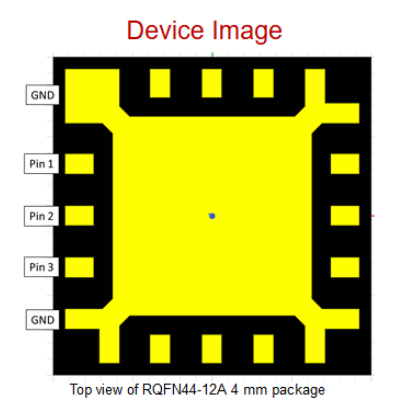
\includegraphics[width=0.5\linewidth]{Figures/RQFN-4-mm.png}
	\caption{RQFN packaging example }
	\label{fig:rqfn-example}
\end{figure}

\subsection{Flip Chip as a packaging option}

Flip chip, also known as controlled collapse chip connection or its abbreviation, C4, is a method for interconnecting dies such as semiconductor devices, IC chips, integrated passive devices and microelectromechanical systems (MEMS), to external circuitry with solder bumps that have been deposited onto the chip pads. This is in contrast to wire bonding, in which the chip is mounted upright and fine wires are welded onto the chip pads and lead frame contacts to interconnect the chip pads to external circuitry.

% ==============================================
% PACKAGING House options
% ==============================================

\subsection{Packaging house options}

Packaging house options are:

\begin{itemize}
	\item TAI PRO
	\begin{itemize}
		\item \href{https://www.taipro.be/production}{\textbf{Website for Production}}
	\end{itemize}
	\item PacTech (IHP has collaboration with them)
	\begin{itemize}
		\item \href{https://pactech.com/wafer-level-packaging-services/}{\textbf{Website for Wafer Level Packaging Services}}
	\end{itemize}
	\item IZM
	\begin{itemize}
		\item \href{https://www.izm.fraunhofer.de/en/abteilungen/wafer-level-system-integration/leistungsangebot/fine-pitch-bumping-for-pixel-detectors.html}{\textbf{Website for Fine Pitch Bumping for Pixel Detectors}}
		\item \href{https://www.izm.fraunhofer.de/en/abteilungen/wafer-level-system-integration/leistungsangebot/single_chip_bumping.html}{\textbf{Website for Single Chip Bumping}}
	\end{itemize}
	\item RJR Technologies
	\begin{itemize}
		\item \href{https://www.rjrtechnologies.com/}{\textbf{Website}}
	\end{itemize}
\end{itemize}

% Additional option is GP technologies

% Belgium company is for packaging

% California houses
% QP technologies
% spectrum semi

\subsection{Packaging terms by AMPLEON}

Packaging is an important element in RF power transistors, influencing both the cost-efficiency and performance of a given device. Since peak powers can vary widely, from as low as 5 W to more than 1 kW, a range of packages is needed to cover every application. The choice of package format (air-cavity or overmolded plastic), often depends on the design requirements, and any \textbf{trade-offs to be made between performance and cost.} \\

\href{https://www.ampleon.com/packages.html}{\textbf{Source for ampleon packaging}}

Types of packaging:

\begin{itemize}
	\item Air-Cavity Ceramic (ACC)
	\item Air-Cavity Plastic (ACP)
	\item Overmolded Plastic (OMP)
\end{itemize}

\subsection{Definition of terms regarding packaging from RJR technologies}

\begin{itemize}
	\item PRQFN - stands for RJR's thermally enhanced \textbf{P}ower ai\textbf{R}-cavity \textbf{Q}uad \textbf{F}lat \textbf{N}o-leads package
	\item Substrate - the base material that holds the circuit and components (chips, wires, and caps) of semiconductor devices
	\item Coupon - a square panel containing a cluster of substrates
	\item Strip - a rectangular laminate panel containing 4 in-line coupons
	\item Laminate - a substrate technology composed of several layers that are pressed/laminated together
	\item Heatslug - a square or rectangular Cu-coin inserted in the middle of the laminate substrate
	\item Via hole - a hole drilled from top to bottom of the substrate and is used for connecting the terminals on top to the corresponding soldering pads underneath
	\item ENEPIG - stands for Electroless Nickel Electroless Palladium Immersion Gold; the die bondable and wire bondable plating on top of Cu-traces in a laminate
	\item Terminal - metal (Cu) traces that serves as connection of the device into the outside world
	\item Solder resist - a thin layer of polymer that is usually applied on top of Cu-traces of the laminate substrate for protection against oxidation, and around the soldering pads to prevent solder bridges from forming between closely spaced solder pads
\end{itemize}

\subsection{Die layout example}

This is an example (estimation) for this PLL project die size and layout:

\begin{figure}[ht!]
	\centering % try to center it
	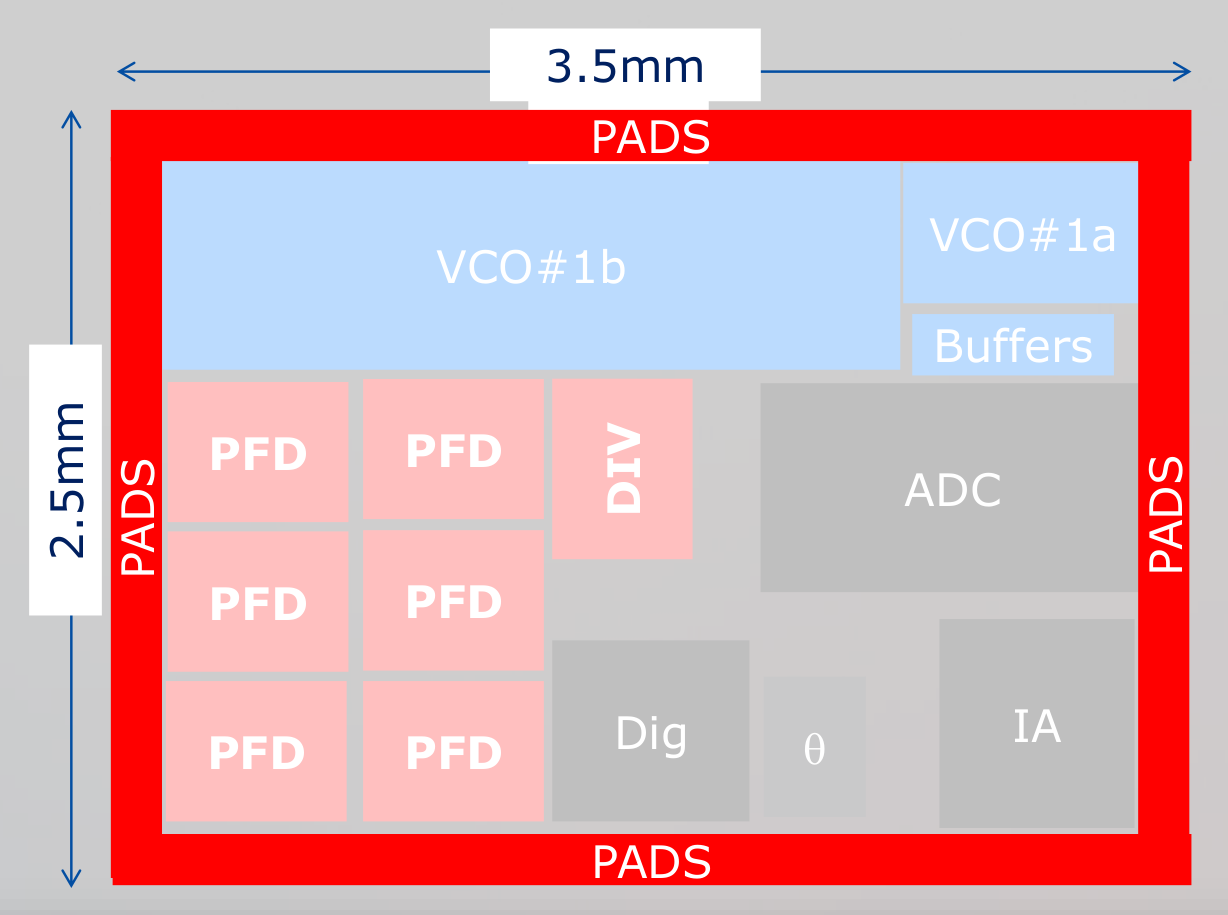
\includegraphics[width=0.5\linewidth]{Figures/die-size-with-pads.png}
	\caption{Die layout with pads }
	\label{fig:die-size-with-pads}
\end{figure}

Also important is the pin count. Absolute minimum is 8 \unit{\milli\metre} x 8 mm.

\begin{figure}[ht!]
	\centering % try to center it
	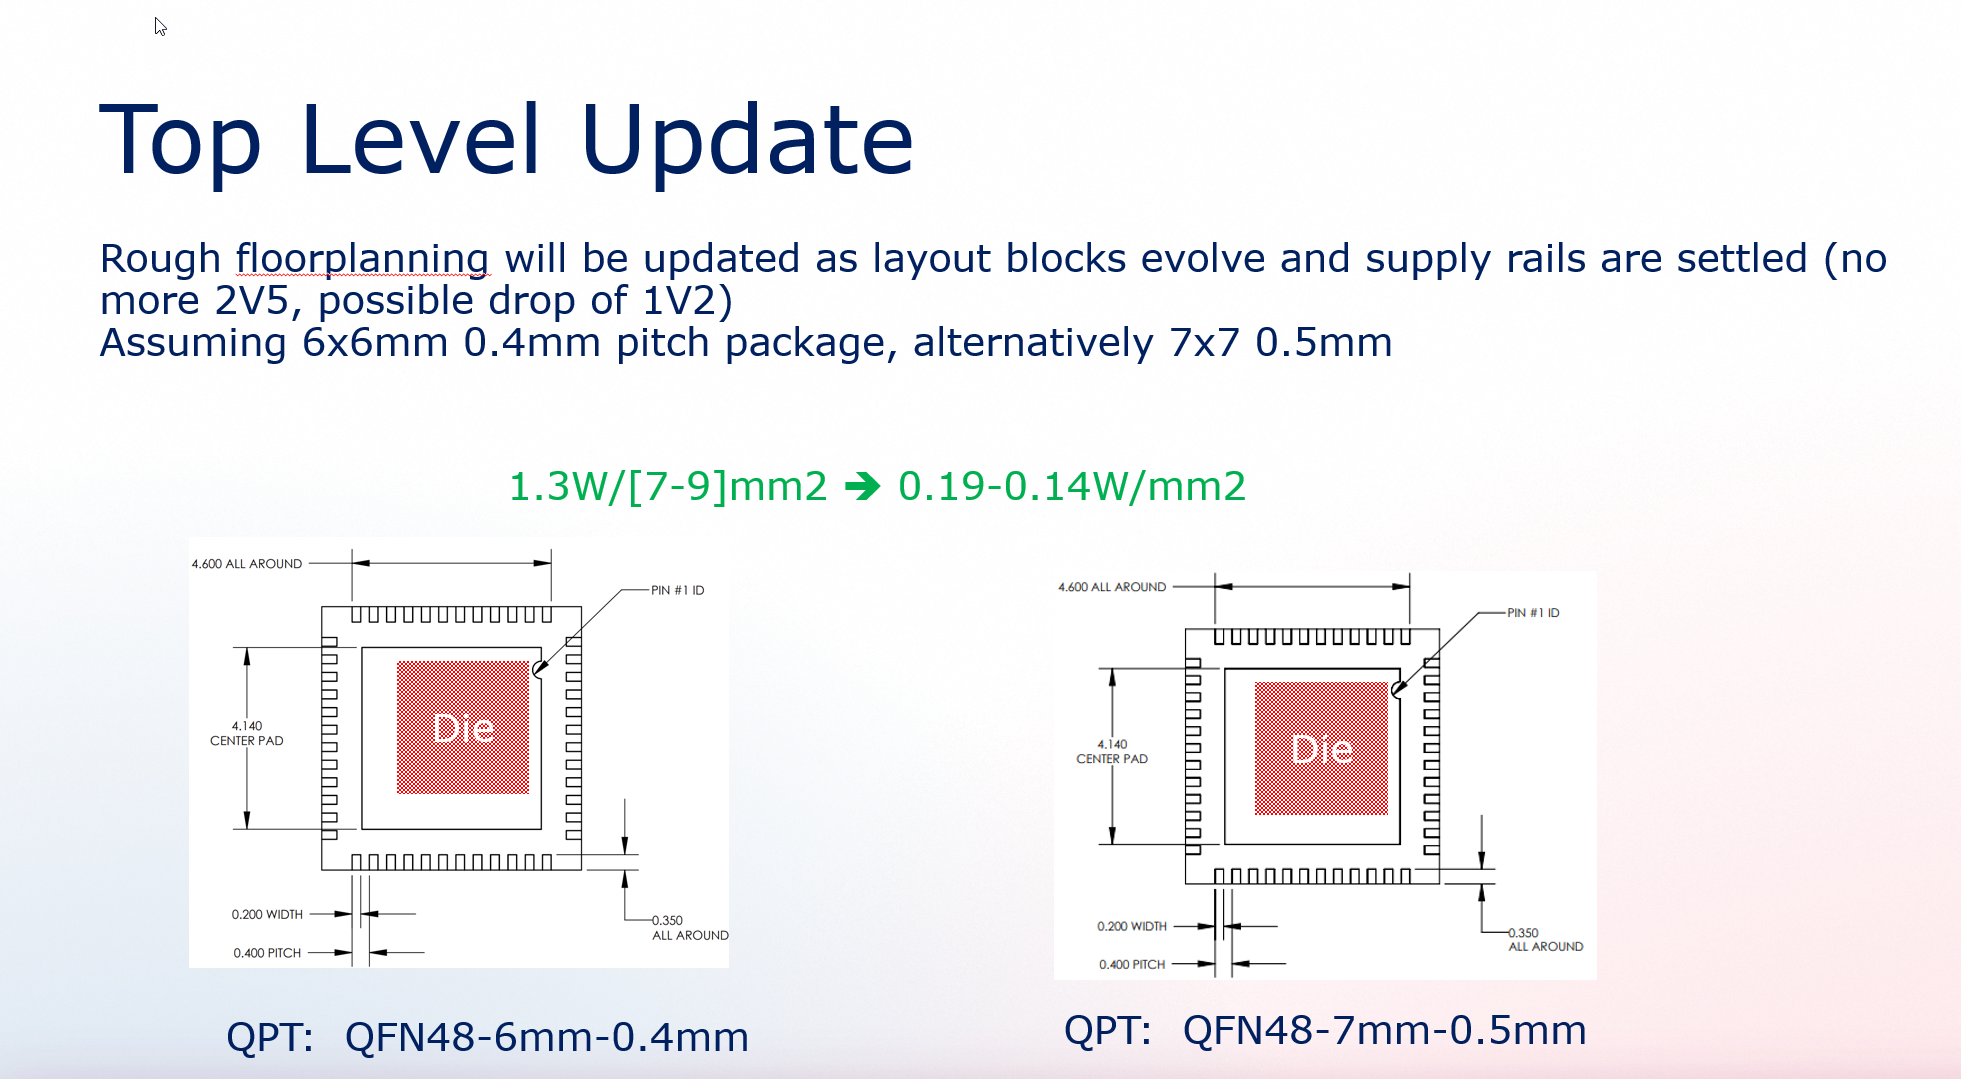
\includegraphics[width=0.5\linewidth]{Figures/powerpoint-toplevel-packaging.png}
	\caption{Top layout and packaging choice}
	\label{fig:powerpoint-toplevel-packaging}
\end{figure}

% ==============================================
% Test Chiup Architecture
% ==============================================

\section{Test Chip Architecture}

Removed CMOS VCO design.

\begin{figure}[ht!] % from Anthony
	\centering % try to center it
	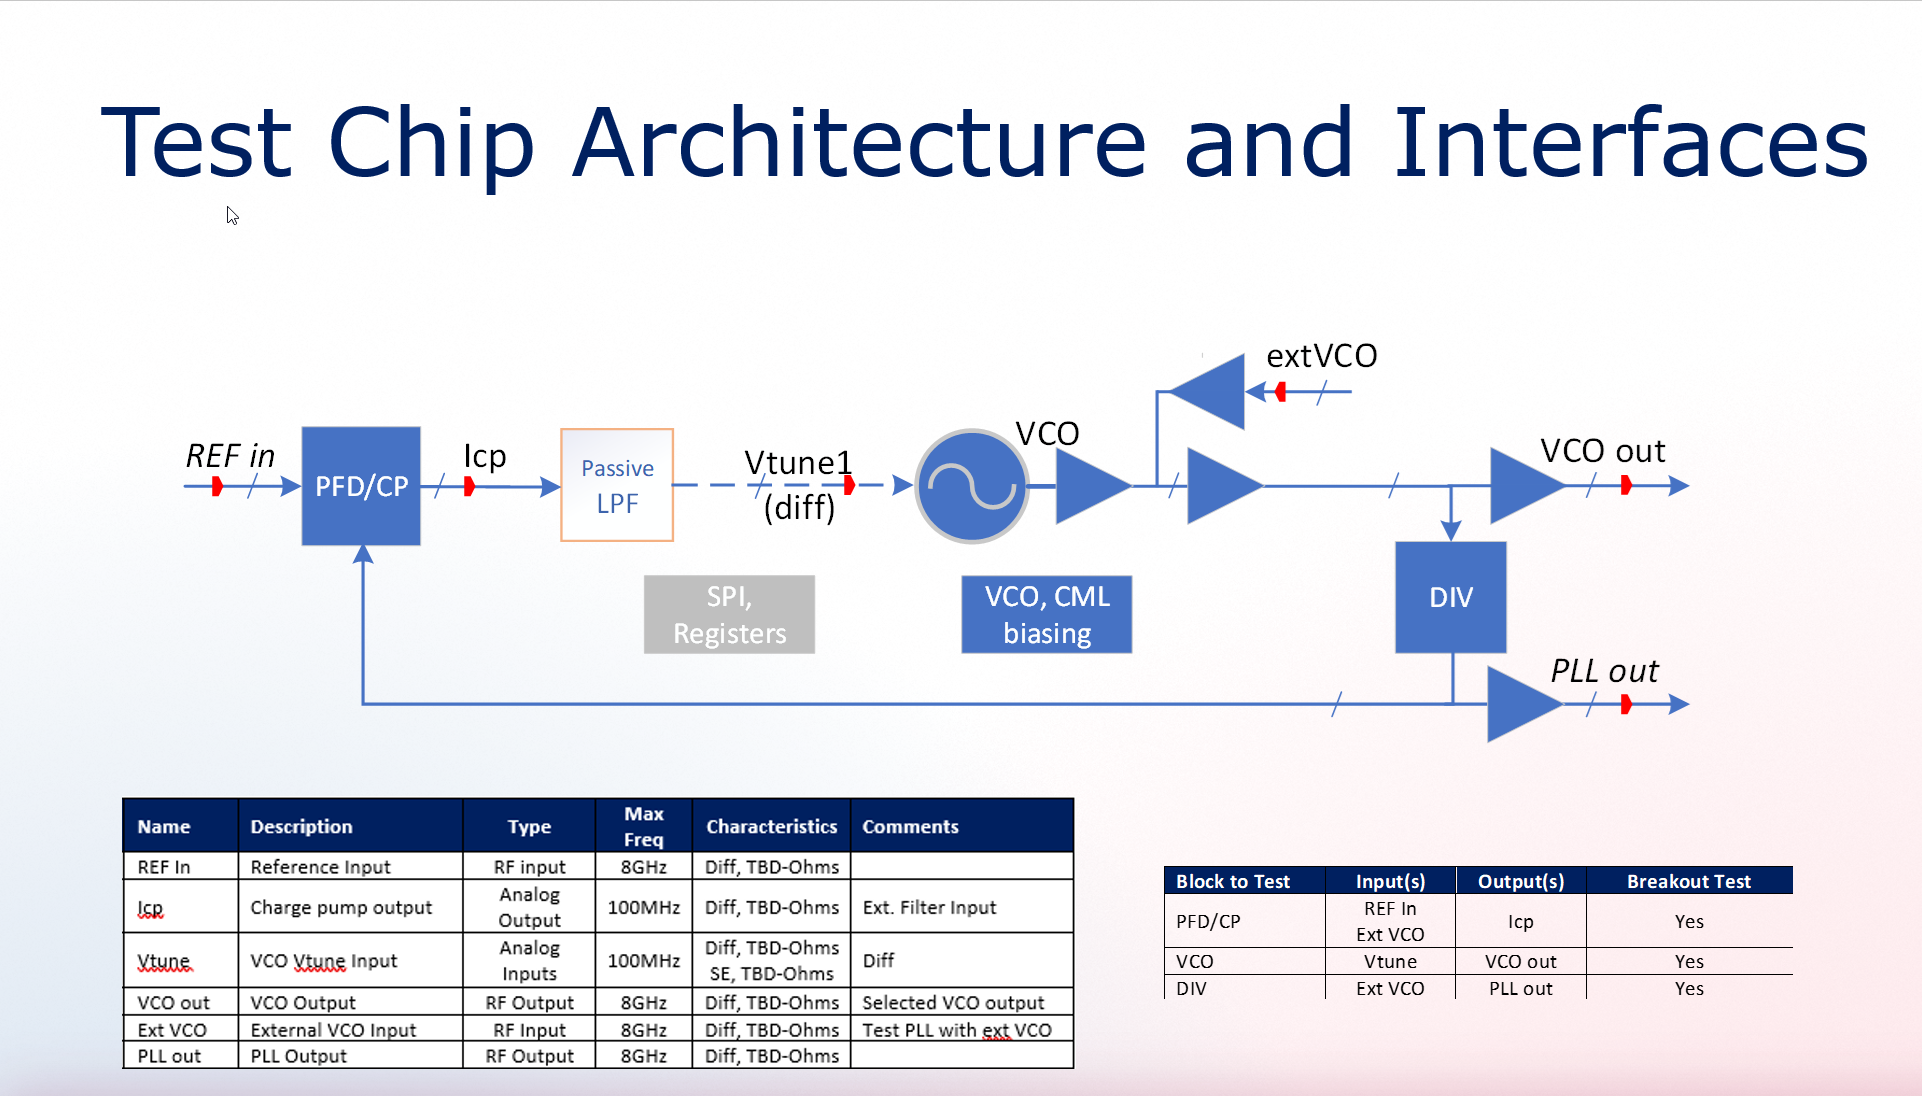
\includegraphics[width=0.5\linewidth]{Figures/test-chip-arch.png}
	\caption{Test Chip Architecture Block Scheme}
	\label{fig:test-chip-arch}
\end{figure}

\subsection*{Identified various risks} % for project plan

\begin{itemize}
	\item VCO phase noise contributors
	\item PFD topology and “blind spots” % not sure how is this tackled?
	\item Discussed design methodology to be finalized in next couple of days
	\item Obtained PDK and discussed risk mitigation strategies % PDK : SG13G2
	\item Started authoring chip system specification
	\item Started project plan with internal and external milestones
	\item Agenda: project progress towards milestones, technical discussion
	\item Review \& signoff of project milestones and plan
	\item Review system specification draft 
	\item Packaging option
\end{itemize}

% ==============================================
% Specification Table
% ==============================================
\newpage
\subsection{PLL overall performance table}

PLL overall performance table:

\begin{table}
	\centering
	\begin{tblr}{
	  row{1}     = {bg = LightCyan},
	  cell{3}{2} = {r=2}{},
	  cell{3}{7} = {r=2}{},
	  cell{5}{2} = {r=2}{},
	  cell{5}{6} = {r=2}{},
	  cell{10}{2} = {r=3}{},
	  cell{10}{6} = {r=3}{},
	  cell{13}{2} = {r=3}{},
	  cell{13}{6} = {r=3}{},
	  cell{17}{2} = {r=4}{},
	  cell{17}{6} = {r=4}{},
	  vlines,
	  hline{1-3,5,7-10,13,16-17,21-23} = {-}{},
	  hline{4} = {1,3-6}{},
	  hline{6,11-12,14-15,18-20} = {1,3-5,7}{},
	}
	\# & Description                                                 & Min  & Typ         & Max  & Units  & Conditions                                        \\
	   & Input Frequency                                             & 1    &             & 8    & GHz    & From Reference generator                          \\
	   & Input Level                                                 &      &             &      & mVppd  & {Accommodating -10..7dBm \\with
	  external BALUN} \\
	   &                                                             &      &             &      &        &                                                   \\
	   & Output Frequency                                            & 1    &             & 8    & GHz    & (range)                                           \\
	   &                                                             &      &             &      &        & (VCO2 range)                                      \\
	   & Output Level                                                &      &             &      & mVppd  & TBD – prefer differential                         \\
	   & Comparison Frequency                                        & 1    &             & 8    & GHz    &                                                   \\
	   & Loop Bandwidth                                              & 1000 &             & 3000 & kHz    & TBD for given configuration                       \\
	   & {VCO noise \\(open loop at 7GHz)}                           &      & -133        &      & dBc/Hz & At 1MHz                                           \\
	   &                                                             &      & -153        &      &        & At 10MHz                                          \\
	   &                                                             &      &             &      &        & At 100MHz                                         \\
	   & REF noise (Test at 7GHz)                                    &      &             &      & dBc/Hz & At 1MHz                                           \\
	   &                                                             &      &             &      &        & At 10MHz                                          \\
	   &                                                             &      &             &      &        & At 100MHz                                         \\
	   & Frequency Division Ratio                                    &      & 1,2,3,4,6,8 &      & -      &                                                   \\
	   & {PLL residual noise\\(Relative to 1GHz,
	  \\excluding VCO)} &      &             &      & dBc/Hz & At 1kHz                                           \\
	   &                                                             &      &             &      &        & At 10kHz                                          \\
	   &                                                             &      &             &      &        & At 100kHz                                         \\
	   &                                                             &      &             &      &        & At 1MHz                                           \\
	   & Settling Time                                               &      &             & 40   & usec   & Target                                            \\
	   & Spurious Rejection                                          & 70   &             &      & dBc    & TBD                                               
	\end{tblr}
\end{table}

% how to calculate the eq tank Rpar

% \section{External and internal milestones}
% Internal are given by anthony
% \subsection{Internal milestones}

% fixed by modifying model files

% \section{Blocks needed} 
% MOVED AFTER VCO


% what does fuses not available mean?

%=======================================================================================================
% VCO THEORY, DESIGN, RESULTS
%=======================================================================================================

\newpage

\section{VCO Theory and Design}

VCO design methodology and specification is split into theory and design.

% ==========================================
% VCO THEORY ONLY
% ==========================================

\subsection{VCO Theory}

% \subsection{VCO phase noise contributors}

\subsubsection*{Phase noise characterisation}

Phase noise represents the short term stability of the oscillator. VCO phase noise contributors listed:

\begin{itemize}
	\item Biasing - voltage and current % , current mirror vs resistor plus voltage reference % voltage and current bias, resistive bias
	\item Quality factor of tank % inductor, capacitor bank and varactor
	\begin{itemize}
		\item Quality factor of inductor
		\item Quality factor of capacitor bank / capacitor bank unit % unit0 and unit1, LSB u_capbank is different
		\item Quality factor of varactor / varactor bank - Differential Tuning vs Single-Ended Tuning 
	\end{itemize}
	\item Core devices contribution 
	\begin{itemize}
		\item The noise sources in a MOS transistor are: thermal noise in the channel, 1/f noise, Noise in the resistive poly gate, noise due to the distributed substrate resistance, shot noise associated with the leakage current of the drain source reverse.
		\item Noise in HBT !?
	\end{itemize}
	\item Supply Noise - since LDO is external, used a plot from LDO documentation 
	\item Amplitude Regulation circuit connection
	\item Peak Detector - negligible simulated 
	\item ISF - Impulse Sensitivity Function - introduces proposed solutions of having non sinewave on tank / or parts of tank (noise sensitivity analysis)
\end{itemize}

\subsubsection*{Noise in HBTs}

Next paragraph(s) are from \href{https://briefs.techconnect.org/wp-content/volumes/Nanotech2005WCM/pdf/1244.pdf}{Physics and Modeling of Noise in SiGe HBT Devices and Circuits}

The ability to simultaneously achieve high cutoff frequency ($f_T$ ), low base resistance ($r_b$), and high current gain ($\beta$) using Si processing underlies the low levels of low frequency 1/f noise, RF noise and phase noise of SiGe HBTs. We will show that the phase noise corner frequency in SiGe HBT oscillators is typically much smaller than the 1/f corner frequency measured under dc biasing.

Origin of Shot Noise - The conventional wisdom is that the power spectral density (PSD) of the base and collector current noises are 2qI or “shot” like. The standard derivation of the magic 2qI shot noise assumes a Poisson stream of an elementary charge q. These charges need to  vercome a potential barrier, and thus flow in a completely uncorrelated manner.

The primary RF noise sources in a SiGe HBT are the noises associated with the dc base and collector currents and the thermal noise of the base resistance. We first discuss physics and models of these noise sources. \\

Lmin is used for HBTs in these low noise applications. 

% non-vco
%=======================================================================================================
% PFD is CML. Has prebuffers, charge pump.
% Should it be characterized near DC like current noise or at higher frequency (att 8 \unit{GHz})
% this was a question for the PFD+CP noise characteristic
%=======================================================================================================


\subsubsection*{Leeson equation}

According to Leeson's Formula, the phase noise in the $\frac{1}{f^2}$ region at an offset frequency $\Delta \omega$ from an oscillation frequency of $\omega_{OSC}$, is given in equation:

\begin{equation}
	PNw(\Delta \omega) = kTR \dfrac{F}{{V_o}^2} {(\dfrac{\omega_{OSC}}{Q \Delta \omega})}^2
\end{equation}

where k, T, R, $V_0$, Q and F are the Boltzmann's constant, the absolute temperature, the equivalent tank parallel resistance, the peak oscillation amplitude, the tank quality factor, and the noise factor, respectively.

Phase noise of VCO according to Leeson's formula behaves like:
\begin{equation}
	PN = 10 * log(K* F^2)
\end{equation}
with change of VCO frequency.

\begin{question}[How are these two equations the same?]
	
\end{question}

\subsubsection*{Time Dependent Dielectric Breakdown}

Concerns on reliability of design, SOA - safe operating area.

\subsubsection*{Test bench for Frequency Pushing and Frequency Pulling}

Frequency pulling is more straightforward than frequency pushing. 

\begin{info}
	Frequency pushing is caused by the VCO's sensitivity to supply voltages. Pushing is a measure of the sensitivity of the VCO output frequency to supply voltage and is expressed in MHZ/volt. The setup	shown in Figure 1 can also be used for this measurement. The supply voltage is set at its nominal	setting and the VCO frequency is recorded for different tune voltages. Next, the supply voltage is increased by 1 bolt and the VCO frequency is measured for different tune voltages as before. Lastly, the supply voltage is decreased by 1 volt from the nominal, and the frequency is measured for different tune voltages once more. At a given tuning voltage, the frequency change due to 1 volt supply voltage change gives the pushing. It may be different at different tuning voltages. A simple program can also automate these measurements
		
\end{info}


\subsubsection*{Frequency scaling and frequency plan}

Formula for normalizing (scaling) phase noise to fundamental (output) frequency:

$PN_{norm}=PN_{meas}-20*log_{10}(\dfrac{freq_{meas}}{freq_{norm}})-20*log_{10}(\dfrac{1}{PNoffset}[MHz])$

Scaling for phase noise in DIV+PFD+CP is different its 10 times log.

\subsubsection*{Suppressed Up-converted Flicker Noise}

From CMOS Differential LC Oscillator with Suppressed Up-Converted Flicker Noise - Aly Ismail, Asad A. Abidi

\begin{info}
	Flicker noise can upconvert around the carrier frequency in many ways, but in practical oscillators two are most important. We illustrate them at work in the conventional differential LC oscillator.
	\begin{itemize}
		\item [1] In the current-limited regime, the tail current governs the steady-state oscillation amplitude. Therefore, 1/f fluctuations in the tail current source (M3) produce low frequency random AM. The random AM envelope modulates the effective capacitance of the tuning varactor, converting AM into FM. The FM sidebands appear as close-in phase noise. 
		\item [2] Flicker noise in the differential pair (M1, M2), modelled by an equivalent noise voltage associated with one transistor in the pair, is injected into the LC resonator as current noise at baseband and at the 2nd harmonic. This cannot account for close-in phase noise. However, the flicker noise also modulates the 2nd harmonic voltage waveform at the tail every half period, inducing a noisy current in CTAIL. After commutation through M1, M2, this current mixes down to the oscillation frequency and presents a fluctuating capacitance across the LC resonator. The resulting random FM upconverts 1/f noise into close-in phase noise.
	\end{itemize}
\end{info}

\subsubsection*{OBSOLETE}

Explored theoretical solutions that are now abandoned.

\subsubsection*{Localized Backside Etching}

Local backside etching (LBE) is a post operation on chip to improve quality (Q) factor of inductor. Affect around 1 kHz offset is 3-4 dBs, and around 0.6 - 1 dB at 1 MHz.

\subsubsection*{Subharmonic Injection Locking}
From what I have seen in papers most promising topology in terms of phase noise is cross-coupled LC VCO class C with potential additional technique of subharmonic injection locking. This is what I plan to try first if no better solutions are provided. Subharmonic injection locking might be too narrowband. % why this became OBSOLETE

\subsubsection*{Tunnel Diode}

% \item [B] I just want to ensure that we're not rebuilding something 1:1 that would benefit from a different structure (thinking about Bosch's wall scanner .. they asked us to turn their discrete circuit 1:1 into an ASIC ... but the central component was a tunnel diode).


% tunnel diode
\begin{info}
	The resonant tunnelling diode (RTD) has been investigated in many high frequency applications, including 712 GHz oscillators [1], voltage controlled oscillators (VCOs) with low power consumption [2], high output power oscillators [3], and also analog-to-digital converters [4].
\end{info}

A tunnel diode is a special type characterized by its ability to exhibit negative resistance. Unlike conventional diodes, which show positive resistance, tunnel diodes can conduct in the reverse bias region under certain conditions. This property makes them invaluable in various electronic applications, especially high-frequency circuits.

\begin{itemize}
	\item [1] Mats Ärlelid, Mikael Nilsson, Gvidas Astromskas, Erik Lind, and Lars-Erik Wernersson, “\href{https://confit.atlas.jp/guide/event-img/ssdm2007/G-5-4/public/pdf_archive?type=in}{High Tuning-Range VCO Using a Gated Tunnel Diode},” Extended Abstracts of the 2007 International Conference on Solid State Devices and Materials, Tsukuba, 2007,-798-G-5-4pp. 798-799
\end{itemize}

\subsubsection*{Emitter and Source Degeneration}

Source capacitive degeneration (CTAIL) is used to improve phase noise performance. 

\href{https://ieeexplore.ieee.org/document/1205652?arnumber=1205652}{Analysis of Emmiter Degenerated LC Oscillators Using Bipolar Technologies} - J. H. C. Zhan, K. Maurice, J. S.Duster, K. T. Kornegay

\subsubsection*{VCO Phase Noise Theoretical Limit}

Regarding VCO phase limit tests: Since noise expresses both in amplitude and phase we could use amplitude regulation to generate the tail current (e.g. using a bipolar current mirror). The problem will then be to minimize noise in the current generator. That could be done with the help of a chopper amplifier. Undesired frequency content may be a new issue, but for a differential design I believe it's solvable. For first tests, an ideal amplifier should come close to that. Maybe a bipolar amplifier doesn't even need that.

\subsubsection*{Trade-off and FoM for VCO Phase Noise and Power Consumption}


Power consumption is not a priority for this project.

\begin{figure}[ht!]
	\centering
	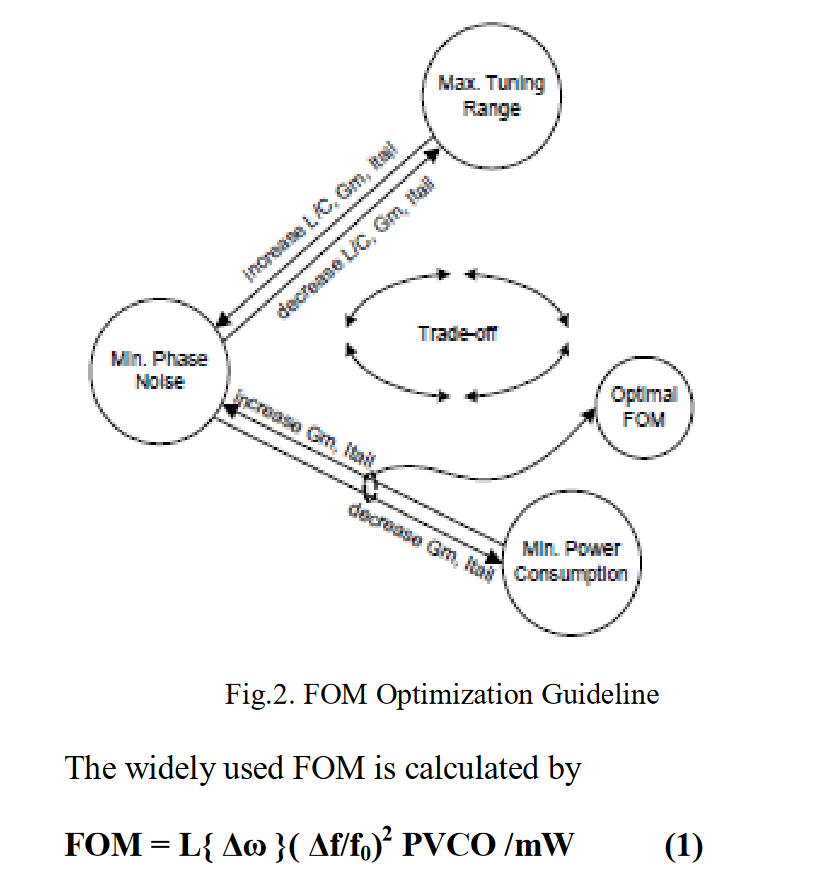
\includegraphics[width=0.5\linewidth]{Figures/vco-tradeoff.png}
	\caption{VCO FoM Optimization and Definition}
	\label{fig:vco-tradeoff}
\end{figure}

\subsubsection*{Substrate integrated waveguide resonators}
% ++++++++++++++++++++++++++++++++++++++++++++++++++++++++++
Substrate integrated waveguide (SIW) resonators are characterized by high quality (Q) factor, easy integration with planer circuits, and lower conductive loss. \\

Oscillators made in SIW :Samundra K. Thapa, Baichuan Chen, Adel Barakat, Kuniaki Yoshitomi, Ramesh K. Pokharel Miniaturized Slot-Loaded SIW Resonator and Its Application to C-band Low Phase Noise Oscillator \\

Z. Chen, W. Hong, J. Chen and J. Zhou, "Design of High-Q Tunable SIW Resonator and Its Application to Low Phase Noise VCO," in IEEE Microwave and Wireless Components Letters, vol. 23, no. 1, pp. 43-45, Jan. 2013. \\

More papers:
\begin{itemize}

	\item[6] F. F. He, K. Wu, W. Hong, L. Han and X. Chen, "A Low Phase-Noise VCO Using an Electronically Tunable Substrate Integrated Waveguide Resonator," in IEEE Transactions on Microwave Theory and Techniques, vol. 58, no. 12, pp. 3452-3458, Dec. 2010.
	\item[7] Z.Yang, B. Luo, J. Dong, T. yang and H. Jin, "Low phase noise oscillator based on quarter mode substrate integrated technique," IEICE Electronics Express, vol. 12, no. 6, pp. 1-6, 2015. 
	\item[8] C. M. Wu, T. Itoh, A. K. Poddar and U. L. Rohde, "A C-band tunable oscillator based on complementary coupled resonator using substrate integrated waveguide cavity," 2014 44th European Microwave Conference, Rome, 2014, pp. 715-718.

\end{itemize}




% \newpage

\subsection{A Noise Circulating Oscillator}

Oscillator phase noise is a fundamental metric that governs a wide variety of design aspects in modern communication and sensing systems [1], [2]

\begin{enumerate} % RF books
	\item B. Razavi, RF Microelectronics, 2nd ed. Englewood Cliffs, NJ, USA: Prentice-Hall, 2011. 
	\item T. H. Lee, The Design of CMOS Radio-Frequency Integrated Circuits. Cambridge, U.K.: Cambridge Univ. Press, 2004.
\end{enumerate}

% ======================================================
% ABOUT CMOS VCO PAPERS
% ======================================================

% Collection of reference papers to read when bored

\subsubsection*{List of SiGe papers}

This is a list of papers regarding the CMOS technology similar to 130 nm collected by Anthony.

\begin{enumerate}
	\item A Stacked-Complementary 5 GHz Oscillator With Even-Only Differential Harmonic Shaping Achieving -150 dBc/Hz Phase Noise at 10-MHz Offset Using Body-Biased Thin-Oxide 22-nm FDSOI
	\item A VCO with Implicit Common-Mode Resonance
	\item A 2.3 - 5-GHz LC-VCO With Source Damping Resistors to Suppress 1/f Noise Up-Conversion
	\item A 6.7-to-9.2GHz 55nm CMOS Hybrid Class-B/Class-C Cellular TX VCO
	\item A 25\% Tuning Range 7.5- 9.4 GHz Oscillator With 194 FoMT and 400 kHz 1/f3 Corner in 40nm CMOS Technology
	\item A Filtering Technique to Lower LC Oscillator Phase Noise
	\item A Low Phase Noise and High FoM Distributed-Swing-Boosting Multi-Core Oscillator Using Harmonic-Impedance-Expanding Technique
	\item A Low Phase Noise, High Phase Accuracy Quadrature LC-VCO With Dual-Tail Current Biasing to Insert Reconfigurable Phase Delay
	\item A Low Phase Noise Oscillator Principled on Transformer-Coupled Hard Limiting
	\item A Noise Circulating Oscillator
	\item Ultra-Low Phase Noise X-Band BiCMOS VCOs Leveraging the Series Resonance
	\item An Ultra-Low Phase Noise Class-F2 CMOS Oscillator With 191 dBc/Hz FoM and Long-Term Reliability
	\item CMOS Differential LC Oscillator with Suppressed Up-Converted Flicker Noise - Aly Ismail, Asad A. Abidi
	\item Design of LC Resonator for Low Phase Noise Oscillators
	\item Even-Harmonic Class-E CMOS Oscillator
	\item Implicit Common-Mode Resonance in LC Oscillators
	\item Third-Harmonic Injection Technique Applied to a 5.87-to-7.56 GHz 65nm CMOS Class-F Oscillator with 192dBc/Hz FOM
\end{enumerate}


\subsubsection*{List of CMOS papers}

% I went through papers that Samuel sent, used the Anthony excel formulas to get phase noise results for comparison.

Franceschin paper has the best noise performance by far. It's made in SiGe 55 nm and using bipolar transistors in core, consumes 500 mA and the output swing is clipped by diode connected bipolars which enables this much current without affecting bipolars operation.

Babaie papers are made in CMOS and are more similar to current design. It utilises step up transformers with different common and differential k factors to decouple capacitor bank from the core and control its drain currents to make a class F2. But I currently don't know how to implement this because I don't have any ideal transformer models with different k factor for differential and common modes.

Ying paper has a similar idea calls it class F23 and also ok results which makes me think this it the most viable idea from all of these papers to try.

% In attachment you can find excel with some extracted information.

\subsubsection*{Paper on YIG VCO}

A Low-Noise Transmission-Type Yttrium Iron Garnet Tuned Oscillator Based on a SiGe MMIC and Bond-Coupling Operating up to 48 GHz Marcel van Delden , Student Member, IEEE, Nils Pohl , Senior Member, IEEE, Klaus Aufinger , Member, IEEE, Christoph Baer , Member, IEEE, and Thomas Musch, Member, IEEE


\begin{info}
	Second, tuneable opto-electronic oscillators (TOEO) use sophisticated optical resonators to tune the output frequency in the microwave range. They offer a high bandwidth of up to more than one octave and low phase noise at the same time [19], [20]. However, TOEOs require at least a laser, an optical resonator, an electrooptic phase or amplitude modulator, a fast photodiode, a delay line as well as a filter, and an amplifier for microwave frequencies. High-performance TOEOs like [19], [20] require even more and sophisticated components. Thus, TOEOs are expensive and complex.
\end{info}

% Only VCO design inquiries
% \begin{itemize}
% 	\item (OBSOLETE) hard-clipped VCO not oscillating at the frequency that is supposed to, drops down to around 1 GHz (example)
% 	\item (OBSOLETE) soft-clipped VCO has more frequency modes - CM and DM resonance
% 	\item Reliability of design, breakdown voltages. TDDB is Time Dependent Dielectric Breakdown. 
% 	\item making a differential varactor instead of the single-ended one
% 	\item What is the name of metal stack process to be used in EM simulations?
% \end{itemize}

% \subsection*{Planning to do at some point}

% \begin{itemize}
% 	\item design a 400 to 500 \unit{pH} inductor (search for a paper that has decent Q factor around 4-8 GHz range) % watch out for electromigration, find the paper that I looked at long time ago
% 	\item design a PTAT bandgap voltage reference to switch the gate from cascaded NMOS to reference
% 	\item make a test bench for frequency pushing and frequency pulling (look at the old VCO project)
% 	\item (DOWNTHELINE) Peak Detector
% \end{itemize}


% Technical Requirements

\subsubsection*{VCO test methods}

\href{https://edisciplinas.usp.br/pluginfile.php/8192379/mod_resource/content/0/VCO-Test_Methods_VCO15-15.pdf}{\textbf{Mini Circuits VCO test methods}} explains how to measure and set up tests for:

\begin{itemize}
	\item output power and frequency
	\item tuning sensitivity and linearity
	\item harmonics and spurious level
	\item frequency pushing
	\item frequency pulling
	\item modulation bandwidth
	\item modern method using a powerful VCO/PLL test system HP4352S
	\item phase noise
\end{itemize}

About modern method: HP has recently introduced a powerful VCO/PLL test system, the HP4352S which is pictured in Figure 4(a). It has built-in low noise power supplies and is available for VCO testing. It measures VCO characteristics such as frequency, tuning linearity, output power, and harmonics as a function of tuning voltage. It can also be used to measure pushing, output power vs. Vcc, phase noise at a given offset vs. VtUne or Vcc, etc. The instrument is user friendly and does not need calibration. A set up using this instrument is illustrated in Figure 4(b). FIGURES NOT SHOWN\\


\newpage

\subsection{Technical requirements}

\begin{table}[ht]
	\centering
	\begin{tabular}{|c|l|c|c|c|c|c|}
		\hline
		& LO Requirements & Note & min & typ & max & Units \\
		\hline
		& \multicolumn{6}{|c|}{\textbf{VCO Requirements}} \\
		\hline
		1 & Full LO range &  & 4000  &  & 8000 & MHz \\ 
		\hline
		1a & Number of cores &  &   & 2 & 4 & / \\ 
		\hline
		2 & Phase Noise at 1 MHz &  &  &  & <-135 & dBc/Hz \\ 
		\hline
		3 & differential Vtune &  & 0.1 &  & Vdd-x & V  \\ % differential
		\hline
		4 & Tuning Sensitivity $K_{VCO}$ &  & ?<30 &  & ?< 50 & MHz/V  \\ 
		\hline
		5 & Pushing & TBD &  &  & 2 & MHz/V  \\ 
		\hline
		6 & Output Voltage p-p & TBD & 0.8 &  & & $V_{p-p}$  \\ 
		\hline
		7 & Load Impedance &  &  &  & 100 & fF  \\ 
		\hline
		& \multicolumn{6}{|c|}{\textbf{VCO and output Buffer}} \\
		\hline
		8 & Output Voltage & TBD & ?0.8  &  &  & $V_{p-p}$ \\ 
		\hline
		9 & Load Impedance & TBD &  &  & ?1000 & fF  \\ 
		\hline
		10 & Harmonic suppression ($2_{nd}$, typ) &  & -15 &  &  & dBc  \\ 
		\hline
		11 & Pulling (14 dB Return Loss, Any Phase) & TBD &  &  & 2 & MHz  \\ 
		\hline
		& \multicolumn{6}{|c|}{\textbf{General Specifications}} \\
		\hline
		12 & Operating Temperature Range &  & -40 &  & 105 & °C  \\ 
		\hline
		13 & Supply Voltage ($\pm 5\%$) &  & 2.375 & 2.5 & 2.625 & V  \\ 
		\hline
		14 & Supply Current &  &  &  & ?20 & mA  \\ 
		\hline
		15 & Shutdown Current &  &  &  & ?10 & $\mu$A  \\ 
		\hline
		16 & Time to Switch Between Cores  &  &  & ?3 & ?5 & ms  \\ 
		\hline
	\end{tabular}
	\label{table-spec-ultra-low-noise}
	\caption{Specification Requirements} 

\end{table}

% FTR - fine tuning range in percentage

\subsection{VCO Design}

\begin{itemize}

	\item What is minimum phase noise that can be obtained with perfect supply, typ process, 25 degC, measured at the VCO output with ideal termination and no buffer
	\item What is the maximum  tuning sensitivity that can be used to obtain the above
	\item What additional techniques need to be explored to improve the above
	\item Perform noise sensitivity analysis like ISF
	\item Discuss CML buffer concept and LDO topologies % LDO will be external
	
\end{itemize}

Previous open points on VCO:

\begin{itemize}
	\item the effects of BSE on phase noise (i.e. is it really needed)
	\item there is no point in using higher resistances than 20 - 30 k$\Omega$ in capacitor bank unit
	\item test voltage and current for HV\_MOSFETs, to test breakdown of mosfets, use software called \textbf{Real Expert} 
	% has to do with SOA (Safe operating area) not being a rectangle
	% find SOA graph in Grujic slides
	\item estimate for drop in phase noise with supply noise and layout and its generous is -120 dBc/Hz % estimate donw by Samuel
	\item to further help needs to review design
\end{itemize}



% I searched relevant papers for VCO 130 nm BiCMOS or similar technologies and frequency range, and haven't found performance even close to 130 dBc @ 1 Mhz offset. 

% \begin{question}[\itshape Based on what was this technology picked for this specification?]
% 	Based on previous feasibility study.
% \end{question}

% \begin{question}[\itshape What is the input reference frequency of PLL? Are there any dividers in PLL?]
% 	Input reference frequency is from 1 GHz to 8 GHz. There are for sure even if the VCO is (4-8 GHz), 2 and 3 dividers are needed.
% \end{question}

% \begin{question}[\itshape Is the input from loop filter single ended or differential?]
% 	It's differential. It also makes more sense for phase noise performance ?!
% \end{question}

% \begin{question}[\itshape How will the PLL lock be detected?]
% 	-
% \end{question}

% Deadbit control is a novel technique to lower settling time.

% Moved to table with technical specifications 

% \begin{question}[\itshape Any estimate for specified VCO output swing?]
% 	-
% \end{question}

% I just realize that BSE should be called LBE (localized backside etch).

\begin{itemize}

	\item [A] another question to the customer regarding the overall system. 8 is a great number for a divider, but maybe a bad choice for a multiplier? I don't know how it is currently implemented, but thinking of diodes/BJT with exponential characteristics we get odd harmonics, using MOS we may get even ones, at least a good 2nd. But 8=2*2*2 and 9 is just 3*3 .. one stage less, and in differential design only 9 seems feasible. In that case I tend to say that a non-sinusoidal output would even help to reduce gain in the multipliers (which also adds noise on top of the multiplication itself). Assuming that the mixer needs amplification, each *2 stage should add more than 6dB PN, leading to about 20dB or more degradation. If they want to have options on that multiplication factor, we could more easily do that in the PLL with dividers (which reduce PN). Ideally we reduce the VCO range to just more than an octave in the highest band of interest and divide the rest?
 
\end{itemize}

% Make two chips (probably for different options for VCO)
% \\
% Test bench to lock PLL, PFD loop filter and VCO.
% \\

% pdk does not support detail inductor modeling.
% \\

% harmonic filter is not included
% \\

% loop bandwidth reallistic that can be achieved internally is from 3 MHz to 100 MHz.
% \\

% up to you if it is 2nd or third order.
% \\






\subsection{Using different models for HBT}

BSIM4 and psp* (not pss), sometimes psp* gives better performance
% TOSEARCH for how "psp" models are really called?

BSIM4, as the extension of BSIM3 model, addresses the MOSFET physical effects into sub-100nm regime. The continuous scaling of minimum feature size brought challenges to compact modeling in two ways: One is that to push the barriers in making transistors with shorter gate length, advanced process technologies are used such as non-uniform substrate doping. The second is its opportunities to RF applications.


% \subsection{Regarding VCO design option 2 results}

% I have simulated pnoise for designs and testbenches Gunther sent me and I don't get the same results.

% I believe simulation using setting multiplenoise that gives phase noise perfrmance that is now being presented is not correct.
% As for multiple different nets it gives very different values, which makes little sense with the topology.
% And when I use only one output noise for pnoise simulation I get much worse results (15-20 dBs), but they are consistent.

% Sorry to bring other people into this, I thought this is important and I wanted to remove myself from these results presented since I also spent some time simulating this design this past week.

% Also for the design Gunther sent me today. The results I got with his testbench:

% These are not normalized results so they are 5-6 dBs lower, but still far from what was expected.

% rfOutputNoise("dBc/Hz" ?result "pnoise")


% \subsection{Tasks regarding the VCO option 2 and 1}

% option 2

% Review VCO option 2 BJT and CMOS options \\
% Review PFD latest results and CP status \\
% Review approach going forward and schedule proposals \\

% Guenter/Aleksandar/Anthime, can we have for each of the blocks (VCO1a, VCO1b, PFD/CP) a status page showing: \\
% performance summary (if different than the VCO comparison table) \\
% any special needs (supply, BSE etc) \\
% projected area \\
% risks so far

\subsection{Problem with discontinuity of RF model}

When simulating design with nmosHVRF models this error appears:

\begin{verbatim}
WARNING (SPECTRE-16780): LTE tolerance was temporarily relaxed to step over a 
		discontinuity in the signal: i_VCO.i_VCO_core.N3:int_INT3. Check the design 
		or use '+diagnose' to get more information.
        Further occurrences of this warning will be suppressed
\end{verbatim}

I changed the model parameter:
\begin{verbatim}
	+ swnqs         =  0.0 * rfmode * 5.0
	In section of sg13g2_moshv_psp_parm.scs/ 
	sg13g2_hv_nmos / model sg13g2_hv_nmos_psp pspnqs103.		
\end{verbatim}

\subsection{30 GHz VCO design}
by Stefan Jović
% with divider by 4 

Performance summary:
\begin{table}[ht]
	\centering
	\begin{tabular}{|c|c|}
		\hline
		Parameter & Typical value \\
		\hline
		Corner & Typical \\
		\hline
		Temperature & 50 °C \\
		\hline
		Amplitude & ~ 550 mVpp \\
		\hline
		Centre Frequency & ~ 30.25 GHz \\
		\hline
		Tuning Range & ~ 0.72 GHz \\
		\hline
		$K_{VCO}$ & ~ 1.45 GHz/V \\
		\hline
		Tuning range voltage & 0.2 V - 0.7 V \\
		\hline
	\end{tabular}
	\label{30GHz-VCO-design}
	\caption{Specification Requirements} 
\end{table}

Some key conclusions in terms of phase noise:

Noise at output of VCO is same as at the output of buffer. Main contributors for VCO output noise is output buffer by performing modulation of VCO tank circuit. Second main contributor is noise in references used to generate VCO current bias and noise in power supply.

Note that current tail bias mirror is using PTAT current.

\begin{question}[\itshape Why is PTAT used?]
	VCO output swing or VCO output freq or sth else?
\end{question}


\subsection{VCO sub blocks and relevant blocks}

List of sub blocks:

\begin{itemize}
	\item VCO core (\# is 8 for BiCMOS)
	\item Differential tuning circuit - varactor (bank)
	\item Capacitor bank
	\item Current or Voltage Bias
	\item Bandgap Reference
	\item Output Buffer
\end{itemize}


% asked for a showcase of source degeneration - response, that it does not actually help

%----------------------------------------------------------------------------------------
%	DESIGN OF VCO TANK
%----------------------------------------------------------------------------------------

\subsection{Design of VCO Tank}

% TOLOOK Design of transformer based tank - Noise Circulating VCO 

\subsubsection{Differential Varactor}
%
2 papers \\

Option 1 is referencing \href{https://ieeexplore.ieee.org/document/1494046?arnumber=1494046}{\textbf{paper}} A 44 \unit{GHz} Differentially Tuned VCO with 4GHz Tuning Range in 0.12 \unit{um} SOI CMOS


\begin{figure}[ht!]
	\centering
	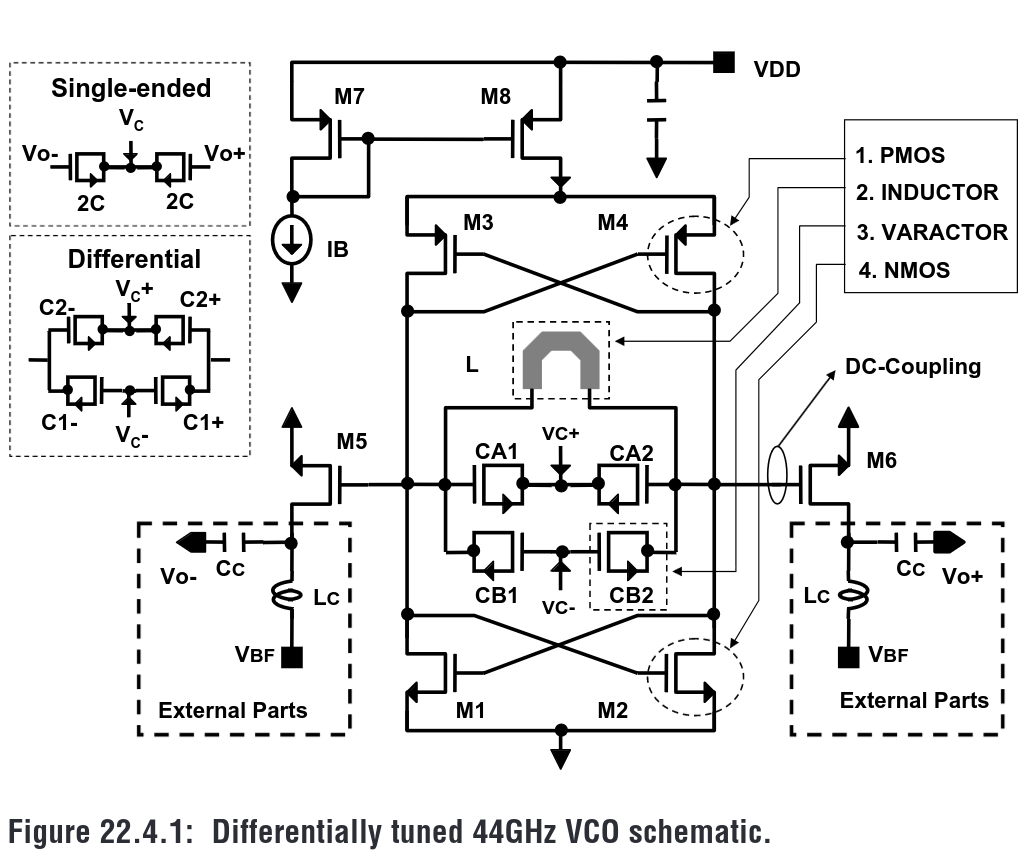
\includegraphics[width=0.5\linewidth]{Figures/diff-var1.png}
	% \caption{Difference between class C and class B}
	\label{fig:diff-var1}
\end{figure}

Option 2 is referencing \href{https://ieeexplore.ieee.org/document/9056968}{\textbf{paper}} A 23-mW 60-GHz Differential Sub-Sampling PLL with an NMOS-Only Differential-Inductively-Tuned VCO
\begin{figure}[ht!]
	\centering
	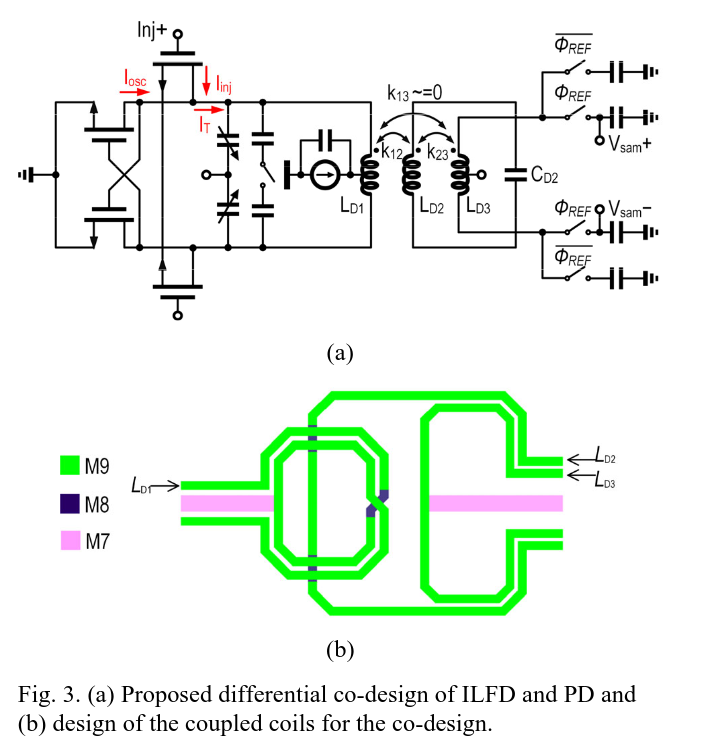
\includegraphics[width=0.5\linewidth]{Figures/diff-var2.png}
	% \caption{Difference between class C and class B}
	\label{fig:diff-var2}
\end{figure}

low Q part of Varactor tuning range: % don't know what i wanted to write

Testbench for comparing differential and single-ended tuning:

\begin{figure}[ht!]
	\centering
	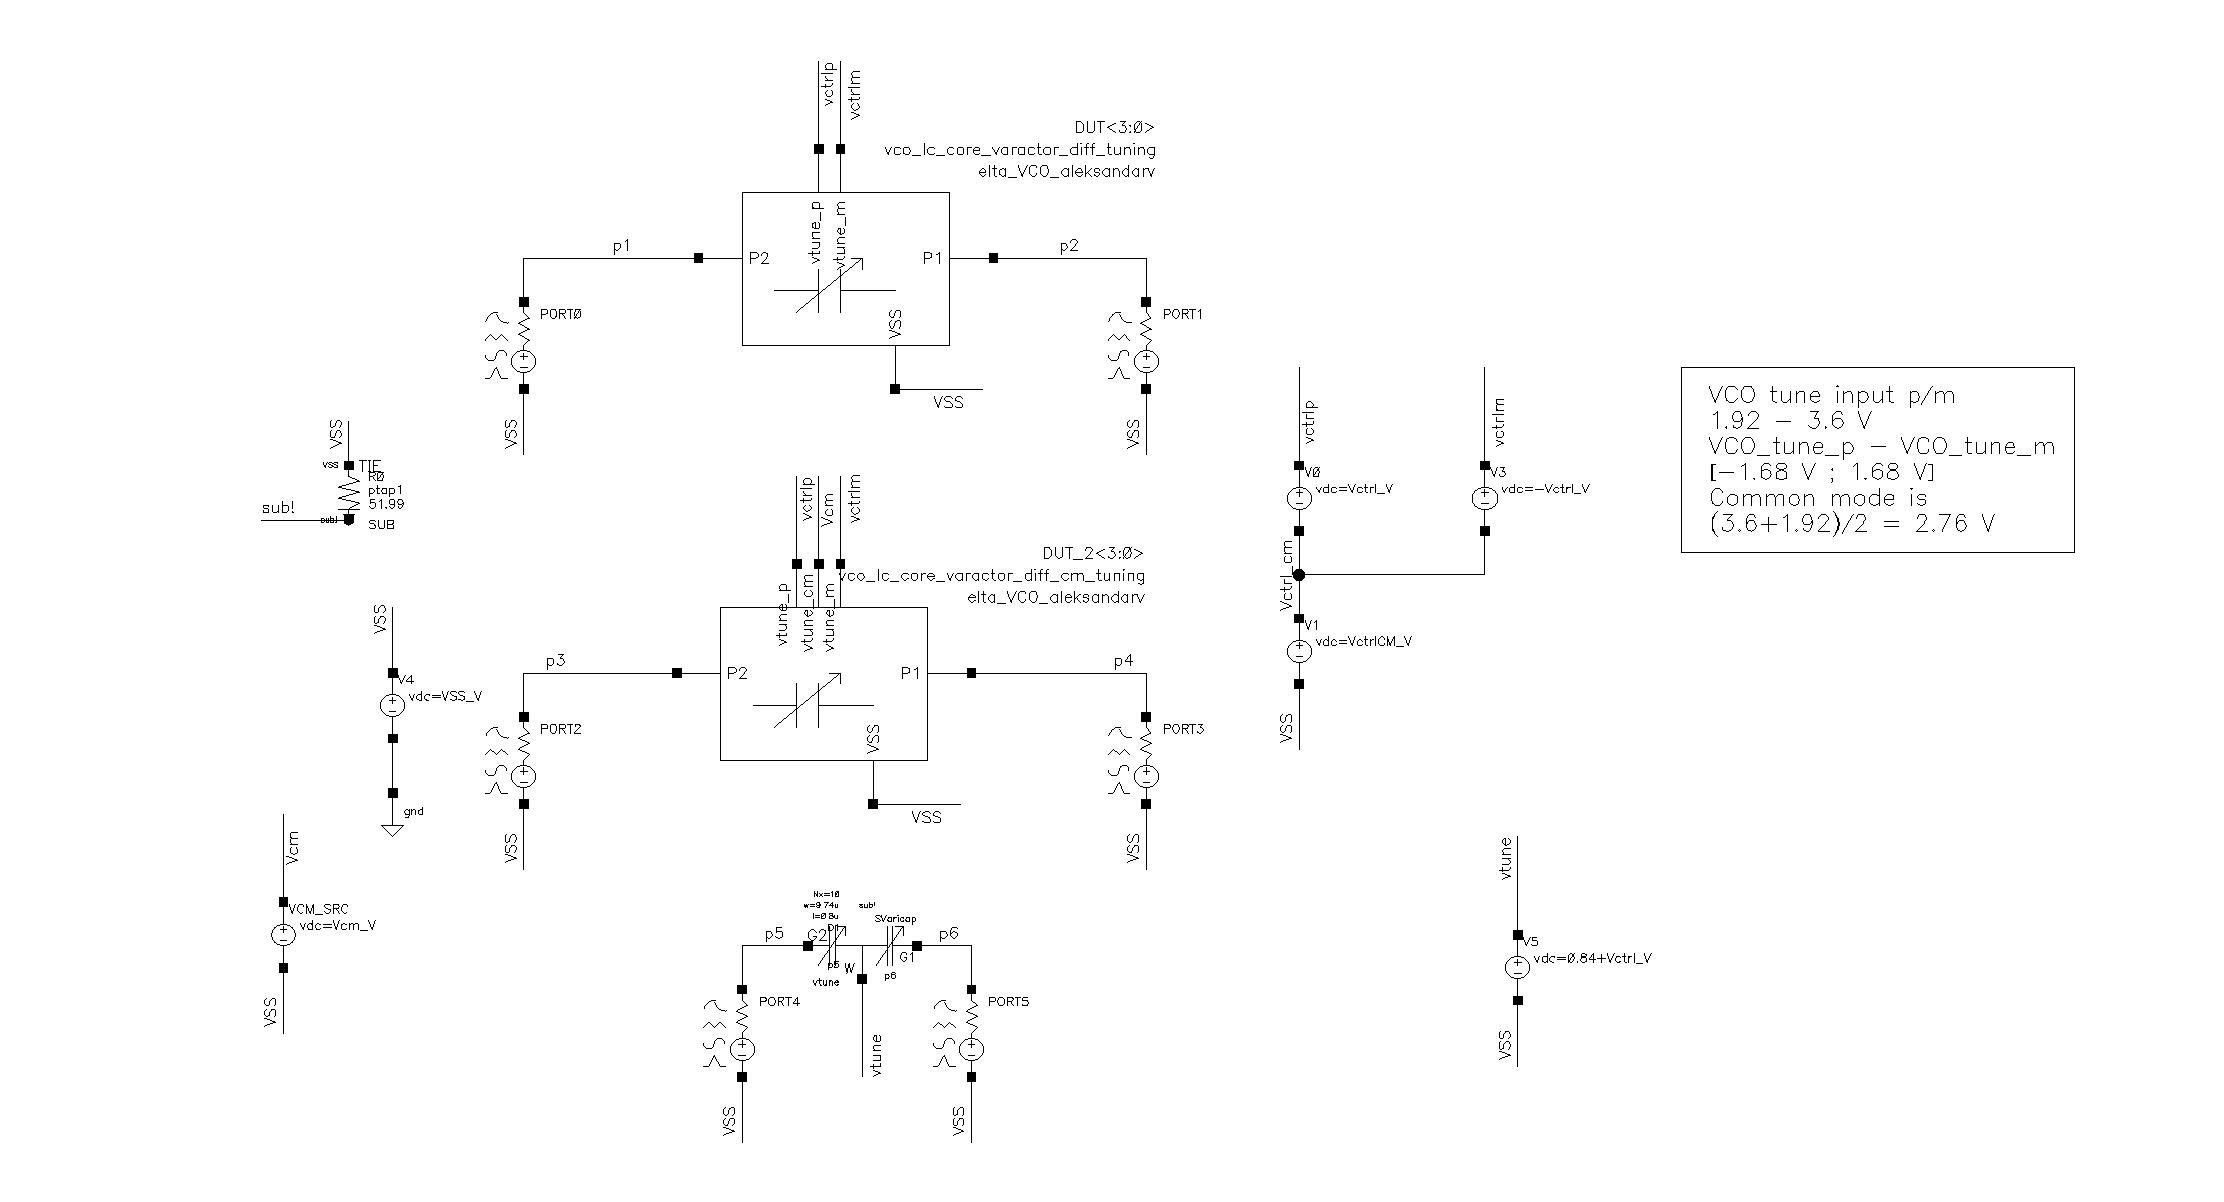
\includegraphics[width=\linewidth]{Figures/cvar-testbench.jpg}
	\caption{Testbench for capacitive varactors}
	\label{fig:cvar-testbench}
\end{figure}

Results of comparative analysis.

\begin{figure}[ht!]
	\centering
	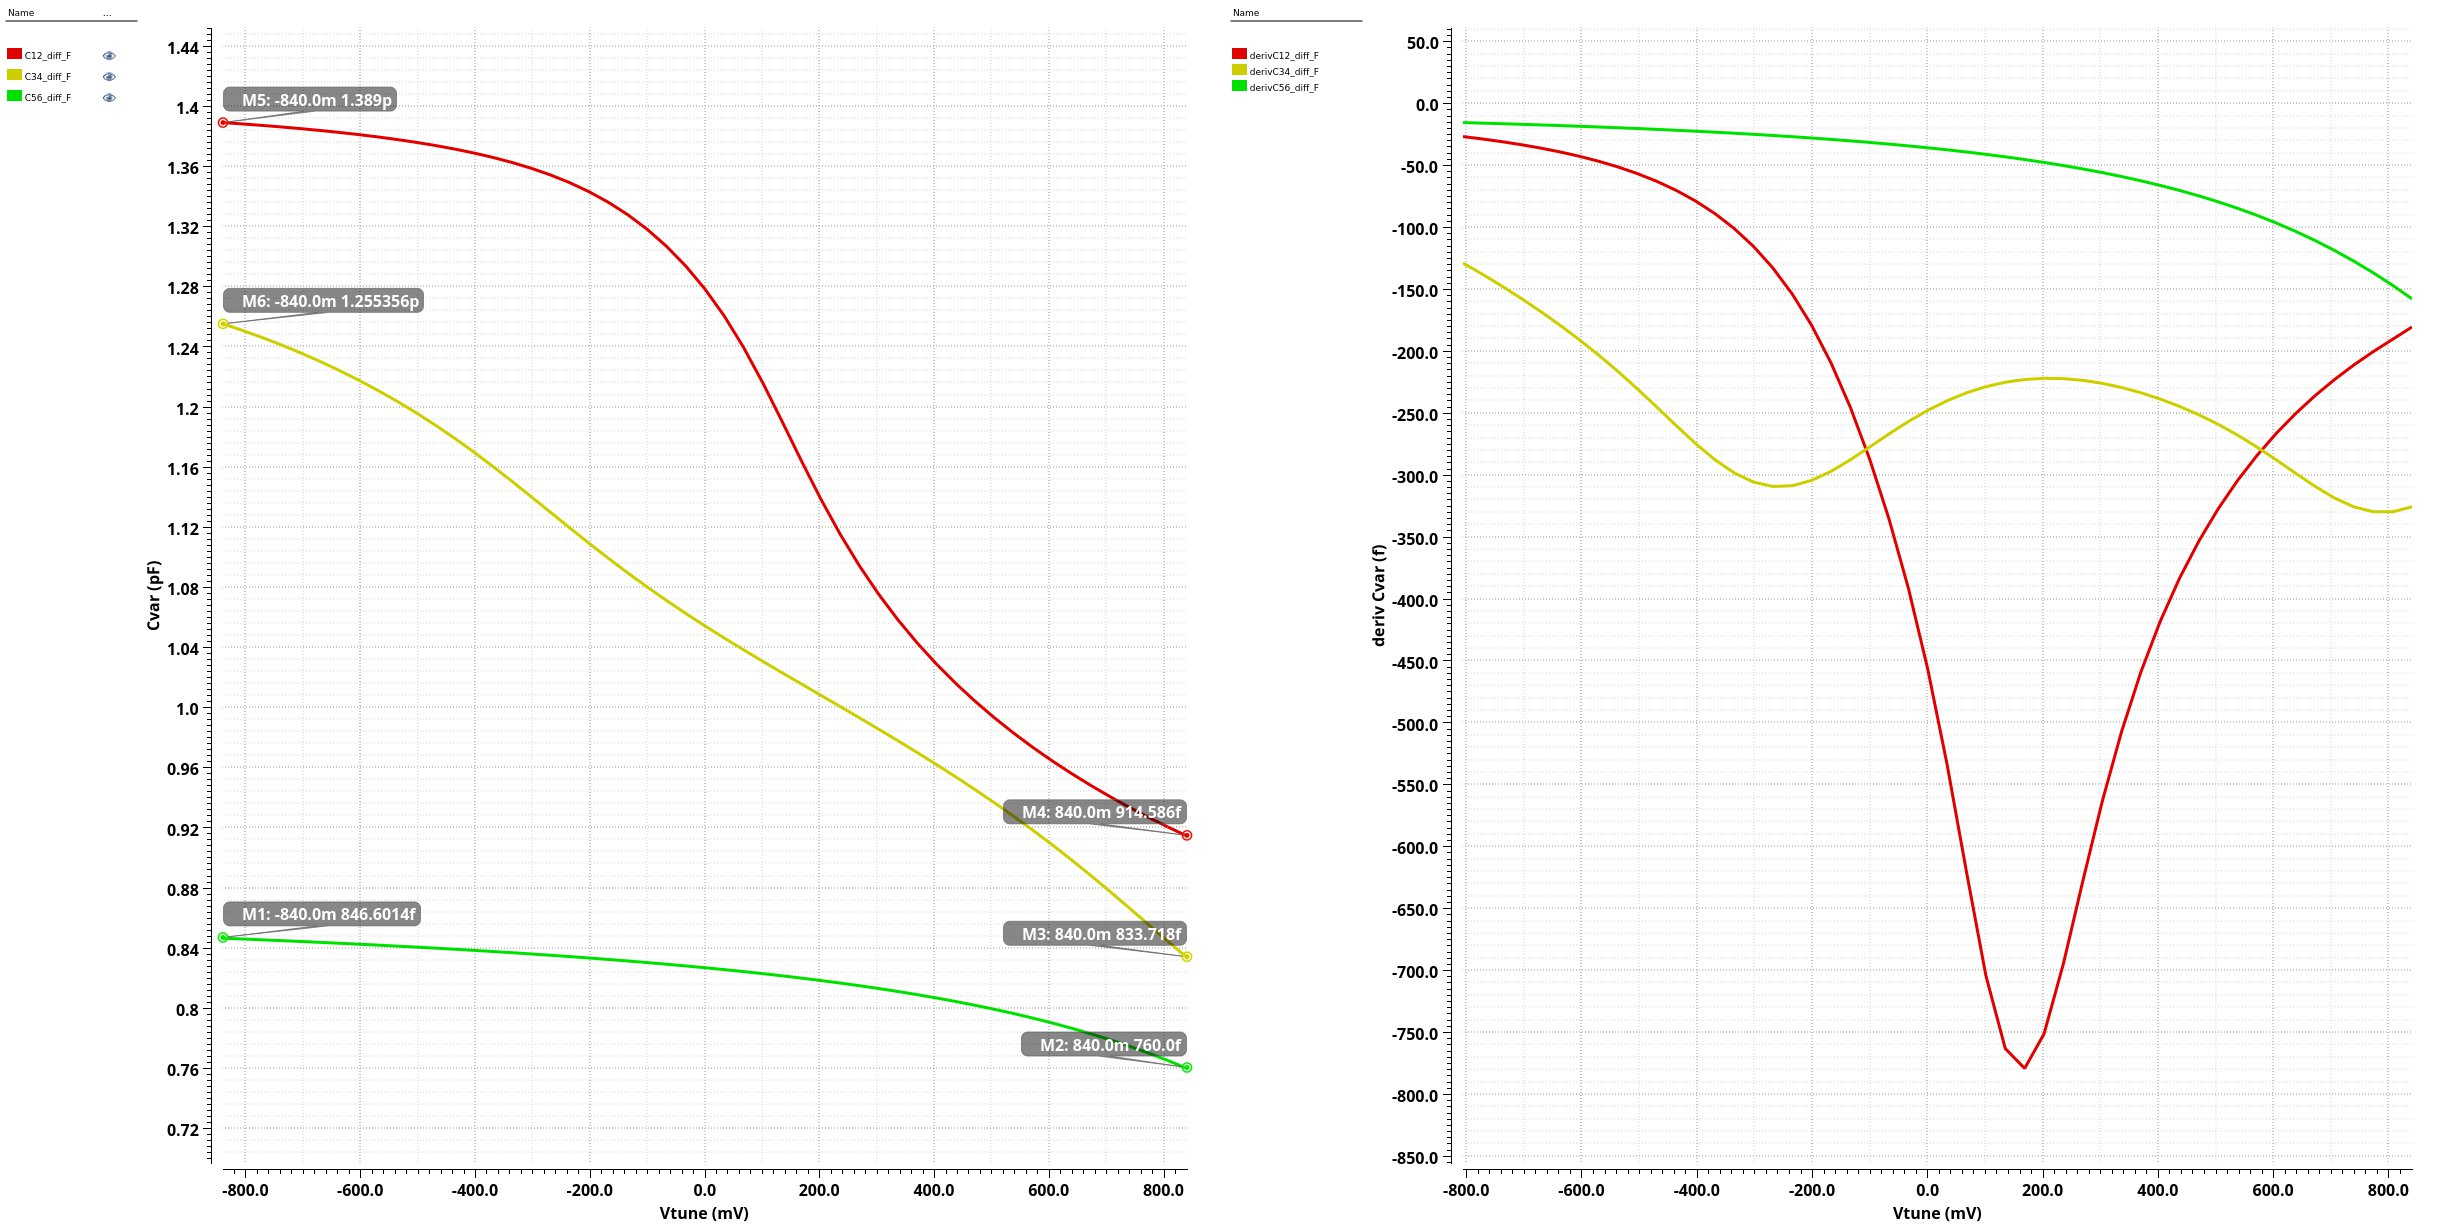
\includegraphics[width=\linewidth]{Figures/cvar-sweep-over-vtune-comparison.jpg}
	\caption{Simulation Results Cvar and deriv(Cvar) over Vtune}
	\label{fig:cvar-sweep-over-vtune-comparison}
\end{figure}

Regarding linearity of differential tuning (I assume you are talking about this), I could not figure this out, and opted for single-ended tuning. The problem is that differential tuning has less capacitance change and inherently loads tank with more capacitance, resulting in lower VCO frequency which results in lower phase noise when normalized to 7 GHz, and also lower tuning range.


Red and yellow are differential "varactors" and green C56 is single-ended. On the left is sweep of tunging voltage to see change in capacitance, on the right derivative of this - indicates KVCO and "linearity".
Yellow is more "linear" than red and  it uses "common mode voltage" Vtunecm = VDD, while red one is the simple one.

This is the schematic for the yellow $C_{34}$ one $vtune_{cm}$ is connected to supply.

Red plot represents this differential "varactor" without cm voltage C12.




% \begin{info}
	
% \end{info}

Q factor is worse for differential tuning vs single-edned tuning.

\subsubsection{Design of Capacitor Bank and CB Unit} % or Banks  

2 Single-ended banks vs Differential capacitor banks

\subsubsection{Design of Inductor}

Electro-magnetic simulator is needed. Technology Parameters if calculations are to be done. Look up the metal stack and info % where to find this

\begin{table}[ht]
	\centering
	\begin{tabular}{|c|c|c|}
		\hline
		Parameter & Value & Unit \\
		\hline
		\hline
		Substrate resistivity & X & $\Omega$-\unit{cm}\\
		\hline
		Substrate thickness & ? & $um$ \\
		\hline
		Silicon dielectric constant & ? & no unit \\
		\hline
		Oxide thickness (M3-Sub) & ? & $um$ \\
		\hline
		Oxide thickness (M3-M2) & ? & $um$ \\
		\hline
		$SiO_2$ dielectric constant & ? & no unit \\
		\hline
		Metal resistivity & ? & $\Omega$-\unit{um} \\
		\hline
		Top Metal (M?) thickness & ? & $um$ \\
		\hline
		Other metal thickness& ? & $um$ \\
		\hline
	\end{tabular}
	\label{tech-param}
	\caption{Technology Parameters} 

\end{table}

Inductor can be also switchable, if we need to improve the crude tuning range.



%----------------------------------------------------------------------------------------
%	NON VCO PARTS OF PLL
%----------------------------------------------------------------------------------------

\section{Non VCO parts of PLL}
%----------------------------------------------------------------------------------------

% non-vco
%=======================================================================================================
% PFD is CML. Has prebuffers, charge pump.
% Should it be characterized near DC like current noise or at higher frequency (att 8 \unit{GHz})
% this was a question for the PFD+CP noise characteristic
%=======================================================================================================

\begin{itemize}
	\item Bandgap PTAT (CTAT?)  % used for
	\item Digital: State Machines, fuses are not available
	\item Digital: Register Bank for VCO bands, cores
	\item DAC, not necessary, could use external
	\item PFD + CP
	\item Passive Differential Loop Filter
	\item Balun is off chip. Multiplexer is high frequency up to 80 GHz - differential amplifier structure.
	\item PLL lock circuit
\end{itemize}

\subsection{Divider}

% Divider probably ratio 12 is not needed.

\begin{itemize}
	\item division rations needed : 1/2/3/4/12
	\item using ecl logic same as PFD
\end{itemize}


\subsection{PFD} % called "blind spots"

PFD topology and blind zone \\
% Question for Anthony and Anthimos

Reset path delay is needed because of dead zone and that is why blind zone was much worse than expected. % so this is a trade-off
\\

\subsection{Loop Filter}

Two options are:

\begin{table}[!ht]
    \centering
    \begin{tabular}{|l|l|}
    \hline
		\rowcolor{LightCyan}
		option 1 & option 2 \\ \hline
        active & passive \\ \hline
        External OpAmp & Diff Charge Pump \\ \hline
        Single-ended Tuning & Differential Tuning \\ \hline
    \end{tabular}
\end{table}

Passive loop filter is chosen because of better phase noise performance.

\subsubsection*{Active Loop Filter Operational Amplifier}

\begin{table}[!ht]
    \centering
    \begin{tabular}{|l|p{100mm}|}
    \hline
		\rowcolor{LightCyan}
        OA Characteristic & Impact/Considerations \\ \hline
        Supply Voltage & The op amp needs to allow the supply range needed for rail-to-rail i/o operation. No obligation to use negative supply rail. \\ \hline
        I/O Common mode range & Output common mode range should allow the VCO to cover the entire tuning range and the input also needs to be rail to rail.* \\ \hline
        Noise Voltage ($nV/\sqrt{Hz}$) & The voltage noise causes phase noise degradation, especially near the loop bandwidth. Smaller is better. \\ \hline
        Minimum Stable Gain & Unity gain stable is preferred. \\ \hline
        Input Bias Currents & This parameter will affect phase detector spurs. Smaller is better. \\ \hline
        Gain Bandwidth Product & As a rough rule of thumb, one would want the gain bandwidth product to be at least 50 times the loop bandwidth. 
		\\ \hline
    \end{tabular}
\end{table}

\begin{itemize}
	\item [*] This is important even in fixed bias topologies as the input voltage connected to the PLL charge pump output will start at the lower rail on power-up.
\end{itemize}

Some commercial part examples to look into:
\begin{itemize}
	\item OP184
	\item AD820
	\item AD8661 
\end{itemize}

\subsection{OTA}

Example of specification:

\begin{table}[ht!]
	\begin{tabular}{|l|l|l|l|l|}
		\rowcolor{LightCyan}\hline
		Parameter                        & \multicolumn{3}{l|}{Value}                & Unit\\ \hline
			                        & Min & Nom & Max              & \\ \hline
		Supply Voltage $V_{DD}$                 & & 3.3 & & \unit{\volt} \\ \hline
		Supply Ground   $V_{SS}$                 & & 0 & & \unit{\volt} \\ \hline
		Supply Variation                 & -5 & & 5     &   \unit{\percent}        \\ \hline
		Temperature range                & -40 & & +125 & \unit{\degreeCelsius}     \\ \hline
		Common Mode Input Range          & 0.1 & & 3.2 & \unit{\volt}        \\ \hline
		Common Mode Output Range         & 1  & & 2.3    &   \unit{\volt}    \\ \hline
		Gain Bandwidth                   & 30 & &          & \unit{\MHz}\\ \hline
		Common-mode rejection ratio @BW  & 40 & &          & \unit{\decibel}\\ \hline
		Power supply rejection ratio @BW & 40  & &        & \unit{\decibel}  \\ \hline
		Variation of transconductance    & -10 & & +10        & \unit{\percent}     \\ \hline
		Slew Rate                        & 20 & & &  \unit{\volt\per\micro\siemens}   \\ \hline
		Input Voltage Offset             & -100& & 100          &  \unit{\micro\volt}  \\ \hline
		Phase Margin                     & 65 & & &\unit{\decibel}         \\ \hline
		DC Gain                          & 50 & & &\unit{\decibel}       \\ \hline
		Current Dissipation              &  & & 1& \unit{\milli\ampere}         \\ \hline
		Area                             & & & 0.05 & \unit{\milli\metre}     \\ \hline
		Capacitive load                  & & 1 &  & \unit{\pico\farad}           \\   \hline
	\end{tabular}
\end{table}

\subsection{Level Shifters}

Lever shifters are digital circtuits that change the high level of signl. In this case from 3.3 V to 1.2 V and other way around.

\begin{table}[ht!]
	\centering
	\begin{tblr}{
		row{1}     = {bg = DarkCyan, fg = white},
	  row{2}     = {bg = LightCyan},
	  cell{1}{3} = {c=3}{},
	  cell{1}{6} = {c=4}{},
	  vline{1-4,7} = {1}{},
	  vline{-} = {2-3,7}{},
	  vline{2-10} = {4-6,8-12}{},
	  hline{1-4,7-8} = {-}{},
	  hline{5-6,9-13} = {2-9}{},
	}
						  &                      & Schematic &        &        & Extracted &        &        &      \\
	Delay times           & \#                   & bcs       & nom    & wcs    & bcs       & nom    & wcs    & Unit \\
	lvlsh 3p3V to 1p2V    & tq\_1p2\_fall\_s     & 144.5p    & 211p   & 301.8p & 147.1p    & 214.7p & 307p   &  \unit{\s}    \\
						  & tq\_1p2\_rise\_s     & 322.8p    & 504.4p & 815.2p & 328.3p    & 512.8p & 828p   & s    \\
						  & tqc\_1p2\_fall\_s    & 285.2p    & 432.6p & 672.9p & 290.2p    & 439.9p & 683p   & s    \\
						  & tqc\_1p2\_rise\_s    & 94.38p    & 140.7p & 201.6p & 96.26p    & 143.5p & 205.5p & s    \\
	lvlsh 1p2V to 3p3V    & tq\_3p3\_fall\_s     & 298.3p    & 530.2p & 1.544n & 355.1p    & 642.2p & 1.867n & s    \\
						  & tq\_3p3\_rise\_s     & 176.9p    & 357.1p & 1.382n & 196.9p    & 413.8p & 1.688n & s    \\
						  & tqc\_3p3\_fall\_s    & 272.7p    & 472.4p & 1.455n & 315.7p    & 563.3p & 1.786n & s    \\
						  & tqc\_3p3\_rise\_s    & 202p      & 417.1p & 1.476n & 238.8p    & 501.6p & 1.781n & s    \\
	Current consumption   & I\_lsh12\_33\_rms\_A & 69.55u    & 89.78u & 121.7u & 75.13u    & 96.94u & 130.7u & A    \\
	for 100  \unit{\MHz} clock      & I\_lsh33\_12\_rms\_A & 22.01u    & 27.65u & 36.54u & 22.35u    & 28.09u & 37.12u & A    \\
	80 ps 90\%-10\% input &                      &           &        &        &           &        &        &      
	\end{tblr}
\end{table}

Example paper for level shifters 
\href{http://leda.elfak.ni.ac.rs/publications/pdf/Conferences/2015/Etran/Low-power%20And%20High%20Speed%20High-to-Low%20level%20Shifter.pdf}{[pdf] High2low Level Shifter}

\section{Supply Regulation}

Needed to reduce the number of supplies.

\subsection{LDO - Low Drop Out Regulators}

Is external filter (capacitor) needed?

\subsection{Bandgap}

Are bandgaps always cvt?
PTAT 


\subsection{Ready Bit}

Needs a comparator to check 1.2\unit{V} supply voltage is higer then some level 

% Also interesting idea is to use TIEHIGH, prolly stupid.


\subsection{Serial Peripheral Interface} 

by Rustam and Nikola

% To continue the conversation about SPI. Nikola and I reviewed our reference design and prepared notes and suggestions for the SPI design.
Looking at SPI slave digital core I see that it will be impossible to redesign it manually to 3.3V. First of all, it will be mess for our layout engineers, because there are too many unstructured cells in this design. PnR is going to be a very exhausting job.

As for the register bank, I suppose that we can do it manually due to repetitive structure it will be copy/paste as Guenter mentioned before.
I prepared a block diagram with my design suggestions. In this example I'm using byte addressing according to existing memory allocation.
 
Here I'm assuming IO cells with 3.3V coreside. So, we should put level shifters from 3.3V to 1.2V on SPI ports. If we will have IO cells with 1.2V coreside we could drop out this level shifters group.

Then we have digital core SPI slave on core logic 1.2V that we will design using standard digital flow using genus/innovus and so on. Then we should put other level shifters from 1.2V to 3.3V on register bank control signals. There won't be many of them, only 21 units. Then we have 3.3V supplied register bank.

For register bank we must get some clock to store data. I see 3 options where we can get clock: 

\begin{itemize}
	\item [1.] we can use existing clock SCLK from SPI port, this way is not ideal, but if we have few free pads, we can go this way.
	\item [2.] we can use external clock from pad, it is preferable option.
	\item [3.] we can use internal generated clock from RC generator, but we should design it at first
\end{itemize}

Talking about core supply rails I see two options: external Vdd pad or internal regulator which, as I understand it, we don't have now either. 
First option with external pad is preferable, but again we will need one more pad.

We should decide which way we choose depending on our possibilities and go on.

\begin{figure}[ht!]
	\centering
	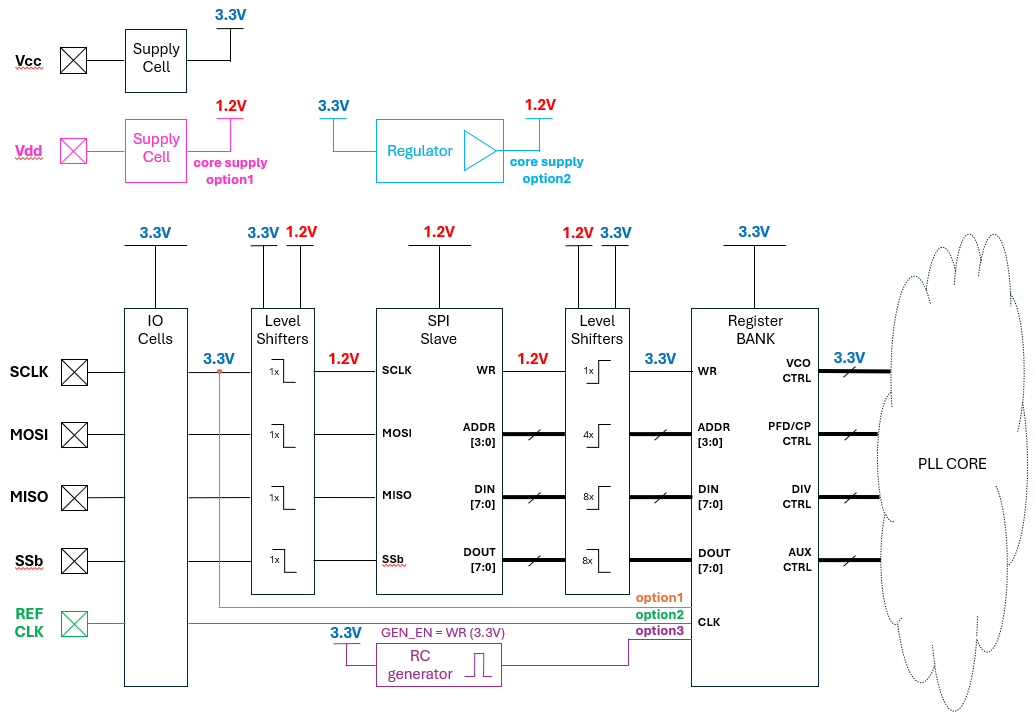
\includegraphics[width=0.5\linewidth]{Figures/spi-suggestion.png}
	\caption{SPI block scheme suggestion}
	\label{fig:spi-suggestion}
\end{figure}


% Nikola and I started working on the SPI. I have one note.
There may be some inconsistency in your proposed requirements. I would like to investigate this to make things clearer.
Your memory allocation assumes byte addressing and has 13 bytes of data. If we are talking about byte addressing, then we need 4 address bits.
But your SPI format proposes 12-bit word addressing and only 3 address bits, plus 1-bit used for R/W annotation.

Test Chip Draft Memory Allocation


\begin{figure}[ht!]
	\centering
	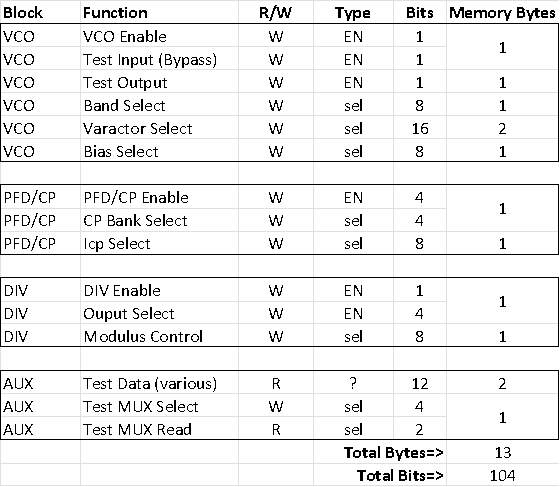
\includegraphics[width=0.5\linewidth]{Figures/test-chip-spi-draft-memory-alloc.png}
	\caption{Test Chip SPI Draft Memory Allocation}
	\label{fig:test-chip-spi-draft-memoery-alloc}
\end{figure}


Basic Format:
Total wordlength: 16bit, 
ADDR, R/W: upper 4bits,
Data: lower 12b for data 
Options:
Adding a test loop for the SPI to verify writes by reading register content back
8 or 12b readback
 
Then I see two options for resolving the issue:

Option 1:
We can use byte addressing according to existing memory allocation. So, we will use 4 address bits to allocate up to 16 bytes.
In this case we should change the command format to: 3 MSB bits - don't care; ADDR - 4 bits; R/W - LSB bit of first byte; DATA - second byte 

\begin{table}[!ht]
    \centering
    \begin{tabular}{|l|l|l|l|l|l|l|l|l|l|}
    \hline
        CMD format & CMD Byte 1 & ~ & ~ & ~ & ~ & ~ & ~ & ~ & CMD Byte 2 \\ \hline
        ~ & 7 & 6 & 5 & 4 & 3 & 2 & 1 & 0 & 7 \\ \hline
        option 1 & x & x & x & A3 & A2 & A1 & A0 & RW & D7 \\ \hline
        option 2 & A2 & A1 & A0 & RW & D11 & D10 & D9 & D8 & D7 \\ \hline
    \end{tabular}
\end{table}


Option 2:
We can use addressing according to your proposed command format. So, we will use 3 address bits to allocate up to 8 words with 12-bit word length.
In this case we should change existing memory allocation table. This is the example:



\begin{table}[!ht]
    \centering
    \begin{tabular}{|l|l|l|l|l|l|l|l|l|l|}
    \hline
        Block & Function & R/W & Type & Bits & \#Bit & \#Word  & ~ & ~ & CMD Byte 2 \\ \hline
        VCO & VCO Enable & W & EN & 1 & 0 & 0 & 1 & 0 & 7 \\ \hline
        VCO & Test Input (Bypass) & W & EN & 1 & 1 & ~ & A0 & RW & D7 \\ \hline
        VCO & Test Output & W & EN & 1 & 2 & ~ & D9 & D8 & D7 \\ \hline
        VCO & Band Select & W & sel & 8 & 3:10 & ~ & ~ & ~ & ~ \\ \hline
        ~ & Dummy & ~ & 11 & ~ & ~ & ~ & ~ & ~ & ~ \\ \hline
        ~ & ~ & ~ & ~ & ~ & ~ & ~ & ~ & ~ & ~ \\ \hline
        VCO & Varactor Select part 1 & W & sel & 12 & 0:11 & 1 & ~ & ~ & ~ \\ \hline
        ~ & ~ & ~ & ~ & ~ & ~ & ~ & ~ & ~ & ~ \\ \hline
        VCO & Varactor Select part 2 & W & sel & 4 & 0:3 & 2 & ~ & ~ & ~ \\ \hline
        VCO & Bias Select & W & sel & 8 & 4:11 & ~ & ~ & ~ & ~ \\ \hline
        ~ & ~ & ~ & ~ & ~ & ~ & ~ & ~ & ~ & ~ \\ \hline
        PFD/CP & PFD/CP Enable & W & EN & 4 & 0:3 & 3 & ~ & ~ & ~ \\ \hline
        PFD/CP & CP Bank Select & W & sel & 4 & 4:7 & ~ & ~ & ~ & ~ \\ \hline
        PFD/CP & Icp Select part 1 & W & sel & 4 & 8:11 & ~ & ~ & ~ & ~ \\ \hline
        ~ & ~ & ~ & ~ & ~ & ~ & ~ & ~ & ~ & ~ \\ \hline
        PFD/CP & Icp Select part 2 & W & sel & 4 & 0:3 & 4 & ~ & ~ & ~ \\ \hline
        DIV & DIV Enable & W & EN & 1 & 4 & ~ & ~ & ~ & ~ \\ \hline
        DIV & CP Bank Select & W & EN & 4 & 5:8 & ~ & ~ & ~ & ~ \\ \hline
        DIV & Modulus Control & W & sel & 3 & 9:11 & ~ & ~ & ~ & ~ \\ \hline
        ~ & ~ & ~ & ~ & ~ & ~ & ~ & ~ & ~ & ~ \\ \hline
        DIV & Modulus Control & W & sel & 5 & 0:4 & 5 & ~ & ~ & ~ \\ \hline
        AUX & Test MUX Select & W & sel & 4 & 5:8 & ~ & ~ & ~ & ~ \\ \hline
        AUX & Test MUX Read & R & sel & 2 & 9:10 & ~ & ~ & ~ & ~ \\ \hline
        ~ & Dummy & R & - & 1 & 11 & ~ & ~ & ~ & ~ \\ \hline
    \end{tabular}
\end{table}

Regarding the clock:
I would prefer not to have an external dedicated clock and also I am a bit worried about an internal clock that may not be fully synchronous to the SPI clock. This leaves the option of using the SPI clock as my preferred solution. 

Regarding the register bank:
I do like your option 1, i.e. using 4 addressing bits. Is everyone else OK with this?

Regarding the 1.2V supply, yes we do not have an internal LDO so we have to rely only to external supplies. Given the very low power consumption at 1.2V I am wondering if we can try any low effort/low cost regulation techniques


%----------------------------------------------------------------------------------------
\section{Commercial Parts}

Commercial parts used as alternative or to augment the design.

\subsubsection*{LMX2592}
LMX2592 High Performance, Wideband PLLatinuTM RF Synthesizer With Integrated VCO

\begin{itemize}

	\item VCO Phase Noise: -134.5 dBc/Hz at 1-\unit{\MHz}
	\item Offset for 6-\unit{\GHz} Output
	\item Industry Leading Phase Noise Performance 
	\item VCO Phase Noise: -134.5 dBc/\unit{\Hz} at 1-\unit{\MHz} Offset for 6-GHz Output
	\item Normalized PLL Noise Floor: -231 dBc/Hz 
	\item Normalized PLL Flicker Noise: -126 dBc/Hz - 49-\unit{\fs} RMS Jitter (12 \unit{\kHz} to 20 \unit{\MHz}) for 6 \unit{\GHz} Output

\end{itemize}

Applications: 

\begin{itemize}
	\item Test and Measurement Equipment
	\item Defence and RADAR
	\item Microwave Backhaul
	\item High-Performance Clock Source for High-Speed
	\item Data Converters
	\item Satellite Communications
\end{itemize}

% Find the commercial part for LDO (Low-dropout regulator)

\subsubsection*{TPS7A8300}

Texas Instruments: TPS7A8300 2-\unit{\ampere},6-\unit{\micro\volt} RMS,RF,LDOVoltage Regulator

\begin{figure}[ht!]
	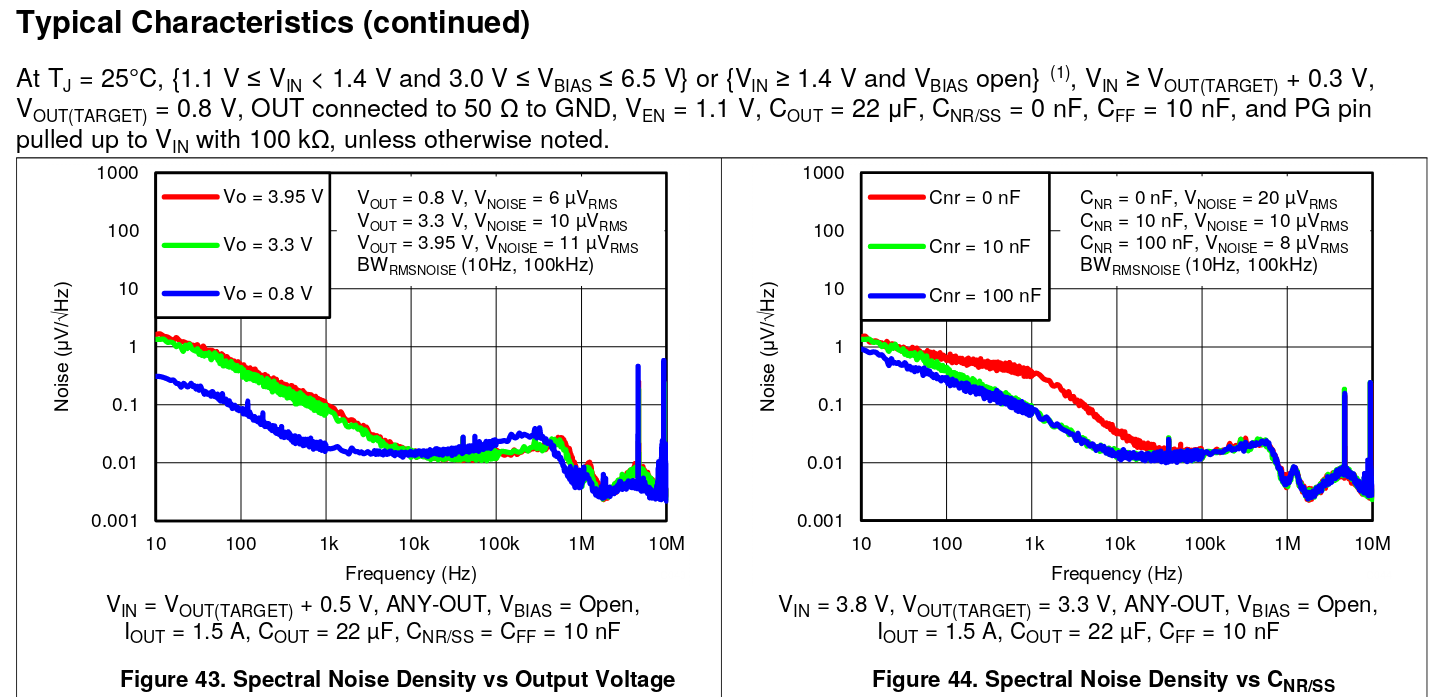
\includegraphics[width=0.5\linewidth]{Figures/LDO-noise-characteristic.png}
	% \caption{Difference between class C and class B}
	\label{fig:ldo-noise-documntation}
\end{figure}


\subsubsection*{HP4352S}

powerful VCO/PLL test system, the HP4352S

\subsection{I/O Baluns}

Presented commercial parts that could be used:

\begin{itemize}
	\item Minicircuits TCM1-83X
	\item Marki Microwave BALH-0012SSG
\end{itemize}





%----------------------------------------------------------------------------------------
%----------------------------------------------------------------------------------------
%----------------------------------------------------------------------------------------
%----------------------------------------------------------------------------------------
\newpage

\section{Old Project}

Old project LO block VCO and VCO Buffer for topcon late 2022. % or time frame

\subsection{Introduction} % Unnumbered section

LO block is LC VCO with internal inductor and fully differential output buffer. Its schematic shall ensure differential connection to the mixer LO input and PLL RF input.

%----------------------------------------------------------------------------------------
\subsection{Technical Requirements}


\begin{table}[ht]
	\centering
	\begin{tabular}{|c|l|c|c|c|c|c|}
		\hline
		\rowcolor{DarkCyan}
		\textbf{\textcolor{white}{\#}} & \textbf{\textcolor{white}{LO Requirements}} &\textbf{\textcolor{white}{Note}}  & \textbf{\textcolor{white}{min}} & \textbf{\textcolor{white}{typ}} & \textbf{\textcolor{white}{max}} & \textbf{\textcolor{white}{Units}} \\
		\hline
		\rowcolor{LightCyan}
		& \multicolumn{6}{c|}{VCO Requirements} \\
		\hline
		1 & Full LO range &  & 6300  &  & 13700 & MHz \\ 
		\hline
		2 & Phase Noise at 300 kHz &  &  &  & <-101 & dBc/Hz \\ 
		\hline
		3 & Vtune &  & 0.1 &  & 1 & V  \\ 
		\hline
		4 & Tuning Sensitivity $K_{VCO}$ &  &  &  & 100 & MHz/V  \\ 
		\hline
		5 & Pushing & TBD &  &  & 2 & MHz/V  \\ 
		\hline
		6 & Output Voltage & TBD & 0.8 &  & & $V_{p-p}$  \\ 
		\hline
		7 & Load Impedance &  &  &  & 100 & fF  \\ 
		\hline
		\rowcolor{LightCyan}
		& \multicolumn{6}{c|}{VCO and output Buffer} \\
		\hline
		8 & Output Voltage & TBD & 0.8  &  &  & V  \\ 
		\hline
		9 & Load Impedance & TBD &  &  & 1000 & fF  \\ 
		\hline
		10 & Harmonic suppression ($2_{nd}$, typ) &  & -15 &  &  & dBc  \\ 
		\hline
		11 & Pulling (14 dB Return Loss, Any Phase) & TBD &  &  & 2 & MHz  \\ 
		\hline
		\rowcolor{LightCyan}
		& \multicolumn{6}{c|}{General Specifications} \\
		\hline
		12 & Operating Temperature Range &  & -40 &  & 125 & °C  \\ 
		\hline
		13 & Supply Voltage &  & 1 & 1.1 & 1.2 & V  \\ 
		\hline
		14 & Supply Current &  &  &  & 20 & mA  \\ 
		\hline
		15 & Shutdown Current &  &  &  & 10 & $\mu$A  \\ 
		\hline
		16 & Time to Switch Between Cores  &  &  & 3 & 5 & ms  \\ 
		\hline
	\end{tabular}
	\label{tab:table-spec}
	\caption{Specification Requirements} 

\end{table}

LO block should have the characteristics given in Table \ref{tab:table-spec}. Due to wide frequency range it is necessary to use switchable capacitor banks. Min and max for supply voltage are not defined in the original document, and time for switching between two cores was defined during the meeting. Currently Full LO range is split between two cores so the requirement should look like this:

\begin{table}[ht]
	\centering
	\begin{tabular}{|c|l|c|c|c|c|c|}
		\hline
		\rowcolor{LightCyan}
		& LO range requirements & Note & min & typ & max & Units \\
		\hline
		1 & High Band core LO range &  & 10000  &  & 13700 & MHz \\ 
		\hline
		2 & Low Band core LO range &  & 6300 &  & 10000 & MHz \\ 
		\hline
	\end{tabular}
	\caption{LO Range Two Core Specification Requirements} 
\end{table}

\begin{question}[\itshape What's the variation for supply voltage?]
	Not defined probably will be the same as the rest of the 
\end{question}


\begin{question}[\itshape $K_{VCO}$ Why is it in the max column? ]
	Didn't get answer for this. It's probably also typical and a value that is expected by the PLL design.
\end{question}

% Footnotes do not work.

Process corners can be found at:

\begin{verbatim}
/tech/tsmc/tsmc40/models/spectre/crn40lp_2d5_v2d0_2_shrink0d9_embedded_usage.scs
\end{verbatim}
% Seems that 

\subsection{Scaldio Design Review}

\begin{question}[\itshape How should calibration be implemented to achieve output voltage peak to peak and minimize noise?]
Is it done for whole PLL?
\end{question}

\begin{question}[\itshape Difference between class-B and class-C vco? ]
	Scaldio uses class-C, so all parasitic capacitances connected to the tail don't matter. Having trouble with observing the currents of drain so cannot check this and compare them. Scaldio looks something between class C and class B because of $V_{gbias}$ voltage and because adding inductor between tail NMOS and switching pair improves phase noise. This is attributed to class B, while class C only needs tail capacitance.
\end{question}

\begin{figure}[ht!]
	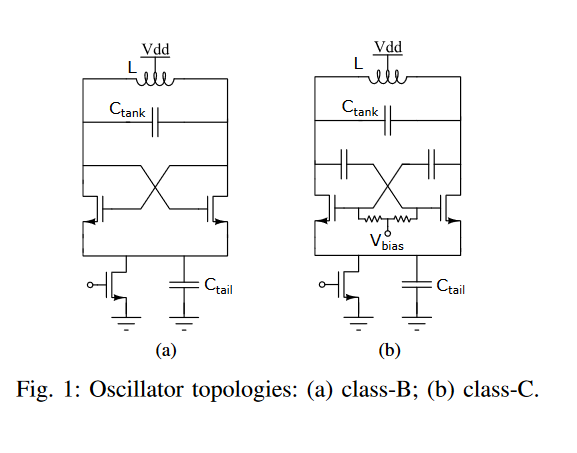
\includegraphics[width=\linewidth]{Figures/class_C_vs_class_B.png}
	% \caption{Difference between class C and class B}
	\label{fig:classC_classB}
\end{figure}

Lowest bit of digital varactor (L0\_PLL\_hbVCO\_Cdig\_SC2B\_VCOS\_SC2C\_PLL) doesn't do anything, isn't even monotonous. Maybe makes more sense when simulating extracted cells. Digital varactor needs to be redesigned, it could lower the Q factor.
Main difference between class B and class C can be observed by investigating their drain currents.

\begin{figure}[ht!]
	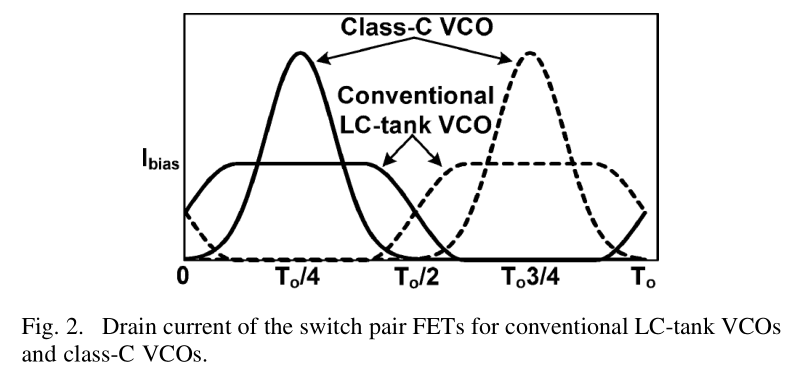
\includegraphics[width=\linewidth]{Figures/drainCurrent_classB_vs_classC.png}
	% \caption{Difference between class C and class B}
	\label{fig:drainCurrent_classB_vs_classC}
\end{figure}

\subsection{Main testbench}

Main testbench covers everything except for frequency pulling and full LO range. The simulation results are obtained at the higher end of the LO range. Phase noise is simulated by pss+pnoise.

\begin{info} % Information block
	With Noise Type=timeaverage and ALL(AM,PM,USB,LSB), you can plot the AM and PM components as well as the total noise. In addition, you can plot phase noise and FM jitter results for oscillators. Plotting is done using the Direct Plot Form.
	\href{https://community.cadence.com/cadence_blogs_8/b/rf/posts/virtuoso-video-diary-noise-simulation-in-spectre-rf-using-improved-pnoise-hbnoise-and-direct-plot-form-options}{\textbf{External link}}
\end{info}

Function of phase noise is simulated for PM noise type.

How to choose beat frequency for autonomous system from forum \href{https://community.cadence.com/cadence_technology_forums/f/custom-ic-design/2661/beat-frequency-in-spectrerf-pss-simulation}{\textbf{thread}}.

\begin{info} % Information block
In an autonomous system (e.g. an oscillator), you turn on the "oscillator" checkbox, and the beat frequency is then the estimated frequency, which gives PSS a starting point to solve for the oscillator frequency. It's important when in oscillator mode to select the outputs of the circuit, which include any subharmonics. In other words, if you have an oscillator followed by a divider, point at the divider output, and give the estimated divided frequency as the beat frequency. Again, this is because you need to solve an integer number of cycles of all the frequencies in the circuit. Note, don't use oscillator mode for circuits which aren't oscillators, since you're then trying to get the simulator to solve for an unknown which is not unknown, which may lead to convergence problems.
\end{info}

Most of the $I_{bias}$ tune digital control is not used for the higher band, so by increasing the number of steps to cover even higher frequencies than the original design finer bias control is needed.


\subsection{Simulation Results for Scaldio design}

Simulated only nominal corner with change for $V_{DD}$ only for frequency pushing simulation. 

\begin{table}[ht]
	\centering
	\begin{tabular}{|c|l|c|c|c|c|c|c|}
		\hline
		\rowcolor{LightCyan}
		& LO Requirements & Note & min & typ & max & Sim(Typ) & Units \\
		% \hline
		% & \multicolumn{7}{|c|}{VCO Requirements} \\
		\hline
		1 & Phase Noise at 300 kHz &  &  &  & <-101 & -98 & dBc/Hz  \\ 
		\hline
		2 & Tuning Sensitivity $K_{VCO}$ &  &  &  & 100 & over & MHz/V  \\ 
		\hline
		3 & Pushing & TBD &  &  & 2  & 279.7 & MHz/V  \\ 
		\hline
		4 & Output Voltage & TBD & 800 &  & & 809.3 & $mV_{p-p}$  \\ 
		\hline
		5 & Harmonic suppression ($2_{nd}$, typ) &  & -15 &  & & -26.78 & dBc  \\ 
		\hline
		6 & Pulling (14 dB Return Loss, Any Phase) & TBD &  &  & 2  & 19.51 & MHz  \\ 
		\hline
	\end{tabular}
	\label{table-ScaldioResults}
	\caption{Scaldio IMEC design Results}
\end{table}

Phase noise changes a lot for different tuning voltages between -90 and -100 dBc/Hz. Phase noise is probably not modeled ok because the VCO doesn't have the connection between current bias tail and the switching pair of VCO as transmission line. That inductance and $C_{tail}$ should resonate at 2$\omega_O$ (tank oscillating frequency), but only in the case of class B oscillator. Check what type is vco oscillator. %This is hard to check because pss\_tran drain currents look wierd.

\newpage

%----------------------------------------------------------------------------------------
\subsection{Q factor of LC tank}

Need testbenches capacitance of tank, varactors and inductor, and for different controls and also corners. Process corners for varactors are the same as MOSFET.

% and of tail (to see how to make it resonate at the double of the oscillating frequency).

\begin{question}[\itshape What kind of chip is it?]
	What kind of inductance is expected to be connected on $V_{DD}$ and $V_{SS}$ pins. This may or may not change the results. Removed all together right now.
\end{question}


\begin{figure}[ht!]
	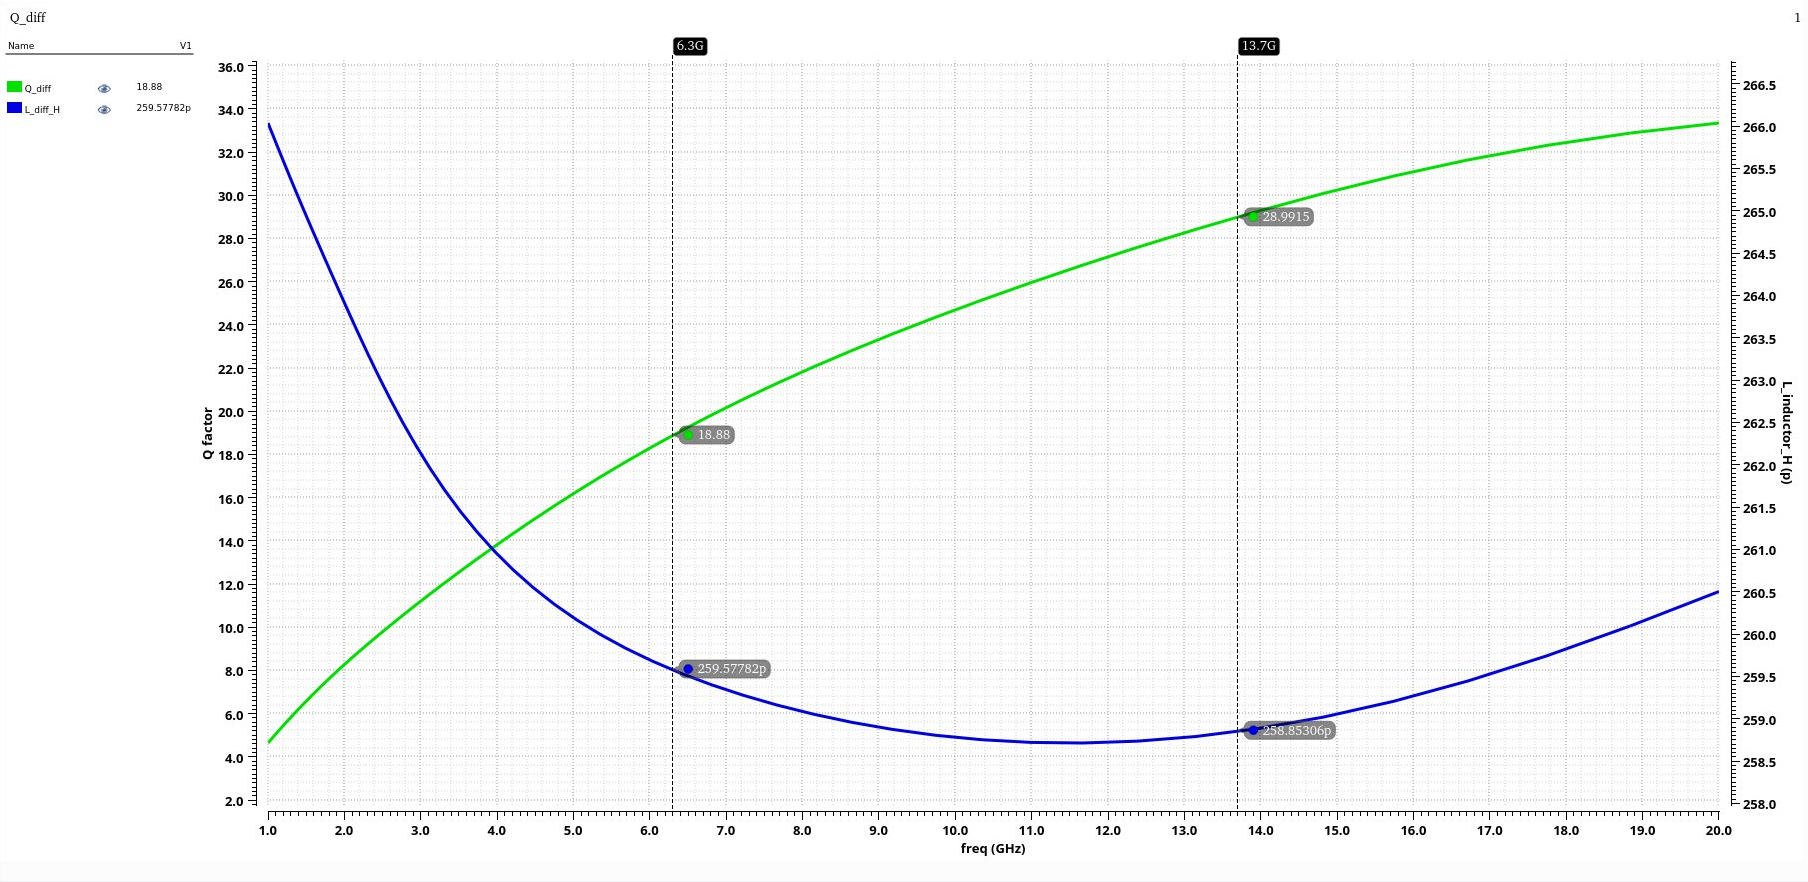
\includegraphics[width=\linewidth]{Figures/QL_inductor.png}
	\caption{Q factor and inductance of L}
	\label{fig:qlinductor}
\end{figure}
Testbench for differential Q and L of the inductor that is EMX simulated is shown in Figure \ref{fig:qlinductor}.

Q factor is better at the higher frequency.

Simulated Q factor of both varactors and inductor. Q factor of digital varactor for lower bit controls is not much better than Q of inductor.

% Differential Q factor of an inductor 

% Zdiff = Z11 + Z22 - Z12 - Z21
% Ldiff = Imag {Zdiff} / 2πf
% Qdiff = Imag{Zdiff } / Real{Zdiff }

Capacitor calculating capacitance and Q factor:

\begin{equation}
	Y_{diff} (im) = imag(ypm('sp 1 1)) + imag(ypm('sp 2 2)) - imag(ypm('sp 2 1)) - imag(ypm('sp 1 2))
\end{equation}

\begin{equation}
	Y_{diff} (re) = real(ypm('sp 1 1)) + real(ypm('sp 2 2)) - real(ypm('sp 2 1)) - real(ypm('sp 1 2))
\end{equation}

Capacitance:
\begin{equation}
	C_{diff} = \dfrac{Y_{diff} (im)}{2\pi f}
\end{equation}

Q factor of capacitor:
\begin{equation}
	Q_C = \dfrac{Y_{diff} (im)}{ Y_{diff} (re)}
\end{equation}

\begin{figure}[h!]
	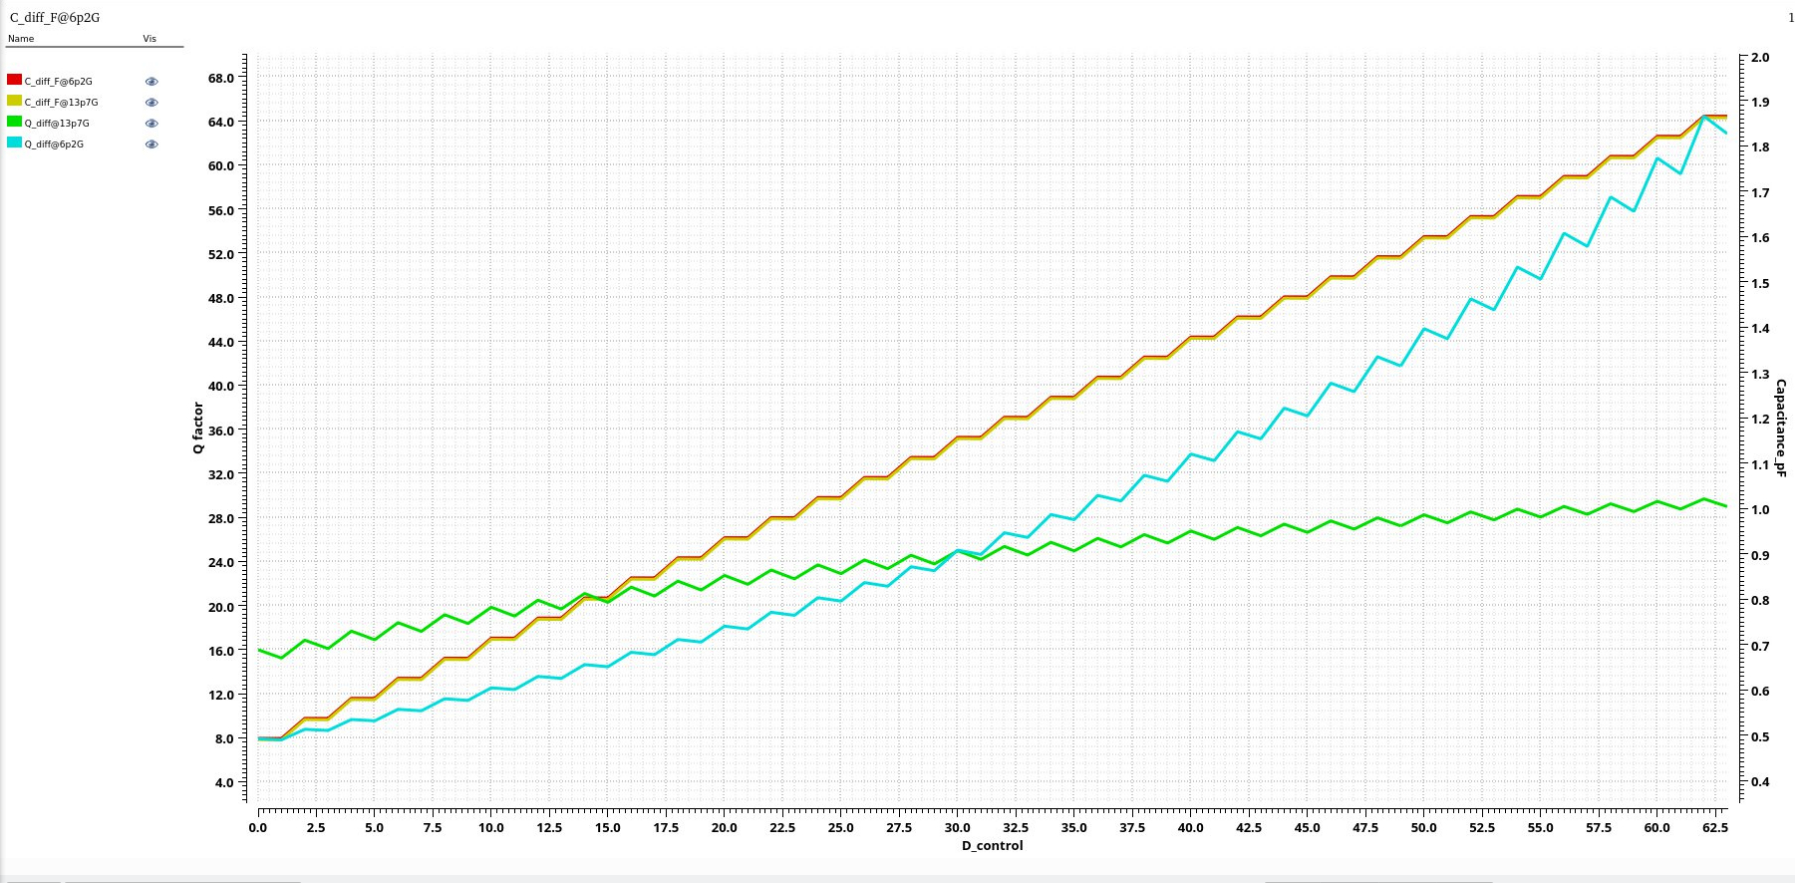
\includegraphics[width=\linewidth]{Figures/Dvaractor.png}
	\caption{C and Q of digital varactor through controls}
	\label{fig:dvaracator}
\end{figure}

More info can be found in  \href{https://ieeexplore.ieee.org/abstract/document/5537949}{\textbf{paper }} A Thorough Analysis of the Tank Quality Factor in LC Oscillators with Switched Capacitor Banks.

Found definitions:

\begin{equation}
	Q_{LC} = \dfrac{1}{R}\sqrt{\dfrac{L}{C}} = \frac{f_r}{\Delta f} = \frac{\omega _r}{\Delta \omega} = \dfrac{\tau _d \omega}{2}
\end{equation}

where $\tau _d$ is group delay.

\begin{question}[\itshape How to calculate group delay using sparam analyis?]
	?
\end{question}

\subsection{Calculating Q factor‚ LC tank by ringing method}

Link to \href{https://www.giangrandi.ch/electronics/ringdownq/ringdownq.shtml}{\textbf{website}} that shows ring down method of calculating Q factor. Not implemented in virtuoso TODO.


%----------------------------------------------------------------------------------------
\subsubsection{Figure of Merit different definitions}

\begin{info} % Information block
	The theoretical maxima for the FoM of an oscillator is given by $FoM=174+20log_{10}(Q)$ dBc/Hz
\end{info}

How to calculate oscillator FoM? Is $Q_L$ factor dominant enough to just equate it with LC tank Q facor.

The widely used FOM is calculated by:
\begin{equation}
	FoM = L\{ \Delta \omega \}( \Delta f/f_0)^2 PVCO [mW]
\end{equation}

Where $L\{\Delta \omega\}$ is the phase noise, $ \Delta \frac{f}{f_0}$ is the ratio between the offset frequency and the carrier, and $P_{VCO}$ is the power consumption of the VCO-core. There is also $FoM^T$ and $FoM_A$ 

\begin{equation}
	FoM^T = FoM - 20 \log (\dfrac{FTR}{10})
\end{equation}

and 

\begin{equation}
	FoM_A = FoM + 10 \log (A)
\end{equation}

where A is area [$mm^2$], and FTR frequency tuning range [$\%$]

Information about digital varactor copied from \href{https://www.doe.carleton.ca/~ddchen/Tutorials/DCO.pdf}{\textbf{External link}}

\begin{info} % Information block
Each bit of MIM varactor contains two MIM capacitors connected differentially with a series switch, two pull-up and two pull-down transistors to effectively turn the varactor between its high and low-capacitance states. Measured intrinsic Q of the MIM capacitor is 80 at 3.6 GHz. When is turned on, i.e., high-capacitance state, the varactor Q drops to 30. When is turned off to be in low-capacitance state, the parasitic capacitance of the MIM capacitor and transistors has an effective of 50. The pull-down transistors set the DC levels for drain and source of at 0 V so that
can be efficiently turned into triode region while the weak pull-up transistors set the DC level to VDDOSC to reduce the parasitic capacitance of thus increasing of the parasitic capacitance. The pull-up pMOS can be implemented by either resistors or transistors. The latter was chosen for silicon area efficiency. Compared to MOS varactors, MIM varactors have a much lower . However, since the differential phase-stability inductor is only 10, the impact of lower varactor is tol erable. When the MIM varactor is at its low-capacitance state, the large DCO internal signal swing and the DC level of 1.4-V supply voltage at source/drain of the pull-up transistors force the drain -nwell junction diodes of the pull-up pMOS to momentarily go into forward-bias condition resulting in a latch-up concern. However, since the forward-bias condition occurs only in 50\% of a 3–4 GHz period, the latch-up phenomenon with the parasitic BJTs can not be triggered.
\end{info}

%----------------------------------------------------------------------------------------
\subsection{Lowering frequency pushing and LDO}

About Frequency pushing from \href{https://www.atlantis-press.com/article/6376.pdf}{\textbf{this paper}}

\begin{info} % Information block
An LC-tank VCO circuit has been implemented in a standard 0.35 $\mu m$ CMOS technology. It is based on a two-transistor biasing structure that improves the performance of frequency pushing and frequency tuning range. Final measurement of proposed structure gives 516 MHz tuning range with 2.278 GHz center frequency and about 0.55$\%$/V frequency pushing in the worst case. The achieved FOM is about -180dBc/Hz, which is very close to the simulated value. This structure is proven to be particularly suitable for achieving low FOM in the VCO circuits having low Q factor LC-tank. Both, the proposed structure and the FOM optimization method, can also be applied to the VCO designs for the applications at higher frequencies, such as 5GHz VCOs for Wireless LAN applications.
\end{info}

\begin{question}[\itshape Can VCO work for lower voltage of 0.9 V?]
	This may be needed if LDO is required because of frequency pushing?
\end{question}

\begin{question}[\itshape Does frequency only happen because of the ripple directly induced by buffers e.g.?]
	Or could it happen because of EM crosstalk?
\end{question}


Is frequency pushing testbench good? Look into this paper. % which paper
Different testbench would be to make a transient change in Vdd and check how much frequency changes.


Results for class C with pmos bias, only dc change of $V_{DD}$:

\begin{center}
	\begin{tabular}{|l|c|c|c|c|c|c|c|c|c|}
		\hline
		Parameter & typical & spec  & min & max & ss -40 & ss 125 & ff -40 & ff 125 & Units \\
		% \hline
		% & \multicolumn{7}{|c|}{VCO Requirements} \\
		\hline
		Frequency Pushing & 43.93 & < 2 &  43.93 & 100.1 & 100.1 & 64.36 & 75.48 & 64.09 & MHz \\ 
		\hline
		Frequency  & 14.6 & > 14.2  & 14.6 & 15.83 & 15.54 & 15.48 & 15.83 & 15.59 & GHz  \\ 
		\hline
	\end{tabular}
\end{center}

This shows some improvement from frequency pushing of 250 - 300 MHz that was observed for the nmos bias of IMEC Scaldio design.

%----------------------------------------------------------------------------------------
\subsection{Changing topology and lowering phase noise}

Decision on why is single sided oscillator chosen instead of double sided oscillator.

\begin{info}
However, if non-negligible parasitic capacitances are found at the tank outputs, the phase-noise performance of the DS-VCO may be seriously degraded, while that of the SS-VCO remains unaffected.
\end{info}

More on the $\frac{1}{f^2}$ Phase Noise Performance of CMOS Differential-Pair LC-Tank Oscillators in \href{https://backend.orbit.dtu.dk/ws/files/3913656/Andreani.pdf}{\textbf{paper}} by Pietro Andreani.


\subsection{Hybrid class C and class B}

\begin{info}
Further, the proposed VCO solves the issue of the hybrid mixed-signal start-up procedure exposed in [8]. The main drawback of this approach is that, if oscillation stops for some unaccountable reason, the VCO can only be restarted actuating again the whole start-up procedure.
\end{info}

Referenced paper is:

\begin{itemize}
	\item [8] J. Chen, F. Jonsson, M. Carlsson, C. Hedenas, and L.-R. Zheng, “\href{https://ieeexplore.ieee.org/document/5951800}{A low power, startup ensured and constant amplitude class-C VCO in \SI{0.18}{\micro\metre} CMOS},” IEEE Microw. Wireless Compon. Lett., vol. 21, no. 8, pp. 427–429, 2011. Dec. 2008.
\end{itemize}


\subsection{Enhanced Oscillation Swing}

Class-C VCO With Amplitude Feedback Loop for Robust Start-Up and Enhanced Oscillation Swing in \href{https://ieeexplore.ieee.org/stamp/stamp.jsp?arnumber=6377236}{\textbf{this paper.}} Phase noise is lowered by lowering $V_{gbias}$, but it makes oscillations start up harder.

\begin{info}
As noted above, the phase noise improves with increasing the oscillation amplitude, which here would mean lowering the gate bias voltage, $V_{bias}$ . Unfortunately, the original class-C oscillator limits the fixed $V_{bias}$ from being set low enough, otherwise the oscillation may not start up. In [11], a high-swing class-C (HSCC) oscillator was introduced, which removed the tail current transistor of the original class-C oscillator [6]. Instead, an automatic amplitude control was introduced to stabilize the oscillation amplitude. In this work, instead of the transformer used in [11], we choose a simple RC bias circuit.
\end{info}

This is from \href{https://www.semanticscholar.org/paper/Dual-Core-High-Swing-Class-C-VCO-design-Kim-Kim/c9551af0809604f76263af49976df9efc213bb8e}{\textbf{paper}} Dual-Core High-Swing Class-C VCO design, and references 


\begin{itemize}
	\item [6] A. Mazzanti and P. Andreani, “\href{https://ieeexplore.ieee.org/document/4684621}{Class-C harmonic CMOS
	VCOs, with a general result on phase noise},” IEEE J.
	Solid-State Circuits, vol. 43, no. 12, pp. 2716–2729,
	Dec. 2008.
	\item [11] M. Tohidian, A. Fotowat-Ahmadi, M. Kamarei, and F.
	Ndagijimana, “\href{https://ieeexplore.ieee.org/document/6045015}{High-swing class-C VCO},” in Proc.
	ESSCIRC, Sep. 2011, pp. 495–498
\end{itemize}


\subsection{Questions about new double feedback}


Amplitude Feedback for Robust start up

% \begin{question}[\itshape What is?]
% 	This may be needed if LDO is required because of frequency pushing?
% \end{question}


\subsection{OTA1 - Start up  and gate voltage bias control}

Referent voltage should be set and controlled around 800 mV. Need tests for OTAs inside for VCO, currently simulated only PM and DC gain, should test different $V_{ref}$ levels.

\subsection{OTA2 - Start up and bias control}

Referent voltage should be set and controlled around 400 mV. Problem with OTA2 loop is amplifying noise into the tail bias current. So the new problem arises as noise shaping in LOOP2 is needed. If a OTA of low uGBW is used than start up is too slow.


%----------------------------------------------------------------------------------------
\subsection{Full LO Range and Frequency Recentering}

% TODO Setup the lb vco, and also setup different testbenches for the highest and the lowest frequency available. Add corner analysis PVT.

TODO Add corners for \textbf{fs sf} and similar. Because the LO range is split on two cores, ideally halved. Results are simulated for process and temperature corners: 

\begin{table}[ht]
	\centering
	\begin{tabular}{|l|c|c|c|c|c|}
		\hline
		Core and Specifictaion & min & max & sim(min) & sim(max) & Units \\
		\hline
		\multicolumn{6}{|c|}{VCO core split} \\
		\hline
		High Band Higher limit & 13700 &  & 15580 & 16190  &  MHz  \\ 
		\hline
		High Band Lower limit &  & 10000 & 10870 & 12460 &  MHz  \\ 
		\hline
		High Band range & 3700 &  & 4710 & 3730 &  MHz  \\ 
		\hline
		Low Band Higher limit & 10000 &   & 13230 & 14120 &  MHz  \\ 
		\hline
		Low Band Lower limit &  & 6300 & 6724 & 8028  &  MHz  \\ 
		\hline
		Low Band range & 3700 &  & 6506 & 6092 &  MHz  \\ 
		\hline
	\end{tabular}
	\caption{LO range specification and simulation for Scaldio LC tank}
\end{table}

Expecting the drop for schematic simulated frequency range, covered range should at least be larger than needed when recentered: 

\begin{equation}
	HBFR = 13700 - 10000 = 3700 < 3730 = 16190 - 12460
\end{equation}

For lower band it's similarily calculated

\begin{equation}
	HBFR = 10000 - 6300 = 3700 < 6092 = 14120 - 8028
\end{equation}

Lower and higher band are assymetrical and they overlap for at least:

\begin{equation}
	HBLBoverlap_{high} = 13230 - 10870 = 2360
\end{equation}

\begin{equation}
	HBLBoverlap_{low} = 14120 - 12460 = 1660
\end{equation}

The worst available frequency digital controlled range is $6092 + 3730 - 1660 = 8162$ MHz which is higher than 7400 MHz.

\begin{question}[\itshape Are the two VCO-s in the same process corner at the same time?]
	Yes. If not than the calculations are wrong.
\end{question}

NOTE: Analog varactor 0-Vt-1 change does not work so it wasn't included. Further frequency recentering after extraction will be needed.

%----------------------------------------------------------------------------------------
\subsection{Pulling testbench and design of VCO buffer}

Needs port at and tuning circuit to keep the reflection at -14 dB. Port of reference impedance 10 k$\Omega$ and portAdapter from rfExamples. S parameter analysis to show if the reflection really is -14 dB? Load impedance increased from 100 fF to 1000 fF. VCO buffer is also needed because of the frequency pulling. Does each core have a buffer or do they share it? first make a buffer than maybe a question.

By adding two buffers from \verb c LO_FDDQ_v6c, \verb c LO_FDDQ_INHB_v5_JCx_scaldio2b  and \verb cLO_FDDQ_BUF_X24 c, frequency pulling drops below 1 MHz. 

So this specification looks fine, testbench shown:


How does portAdapter work?


Frequency pulling mentions coupling (crosstalk) between different blocks on chip and the VCO.
%----------------------------------------------------------------------------------------
\subsection{PTAT and CTAT, the temperature independant Vbias for cascode}

% \verb c c

TODO Simulate and show results of temperature sweep.


%----------------------------------------------------------------------------------------
\subsection{Effect of too high tail capacitance}

\begin{figure}[!ht]
	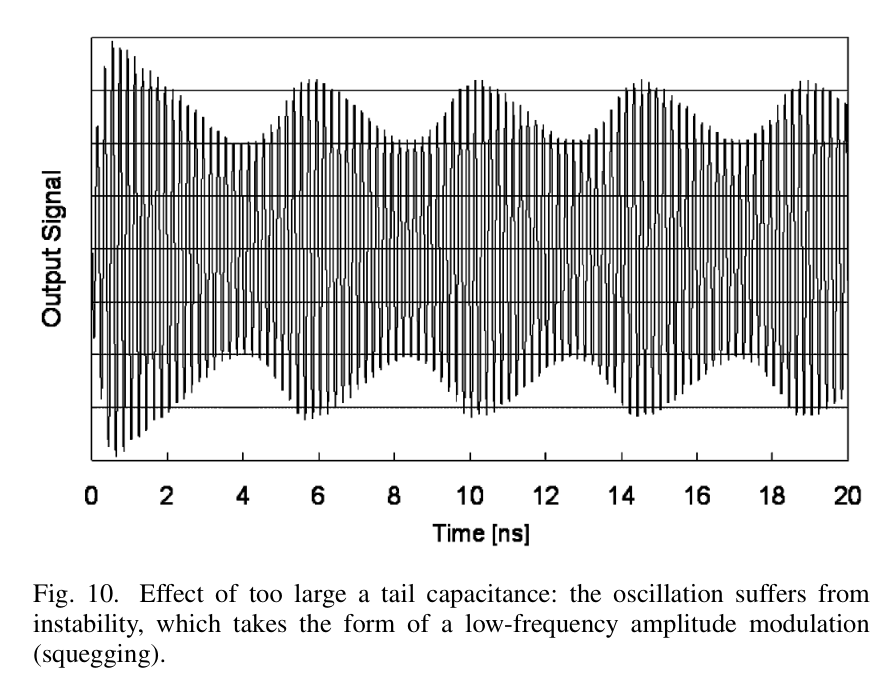
\includegraphics[width=\linewidth]{Figures/squegging.png}
	\caption{Squegging}
	\label{fig:squegging}
\end{figure}

Instability Low frequency amplitude modulation squegging. This was the issue with the original class C with tail current. Is it important for new topology where current bias is PMOS.

\subsection{PLL theory - PLL Lock Detect and calibration}

About PLL Lock Detect:

\begin{info} % Information block
	The ability for a PLL to reliably indicate when it is in lock is critical for many applications. An ideal lock detect circuit gives a high indication when the PLL is locked and a low indication when the PLL is unlocked. When VCO calibration finishes it can be indicative if the lock is detected. 
\end{info}

PLL VCO calibration usually goes as amplitude frequency and then amplitude calibration, or the other way?

Divide and Conquer algorithm


\begin{figure}[!ht]
	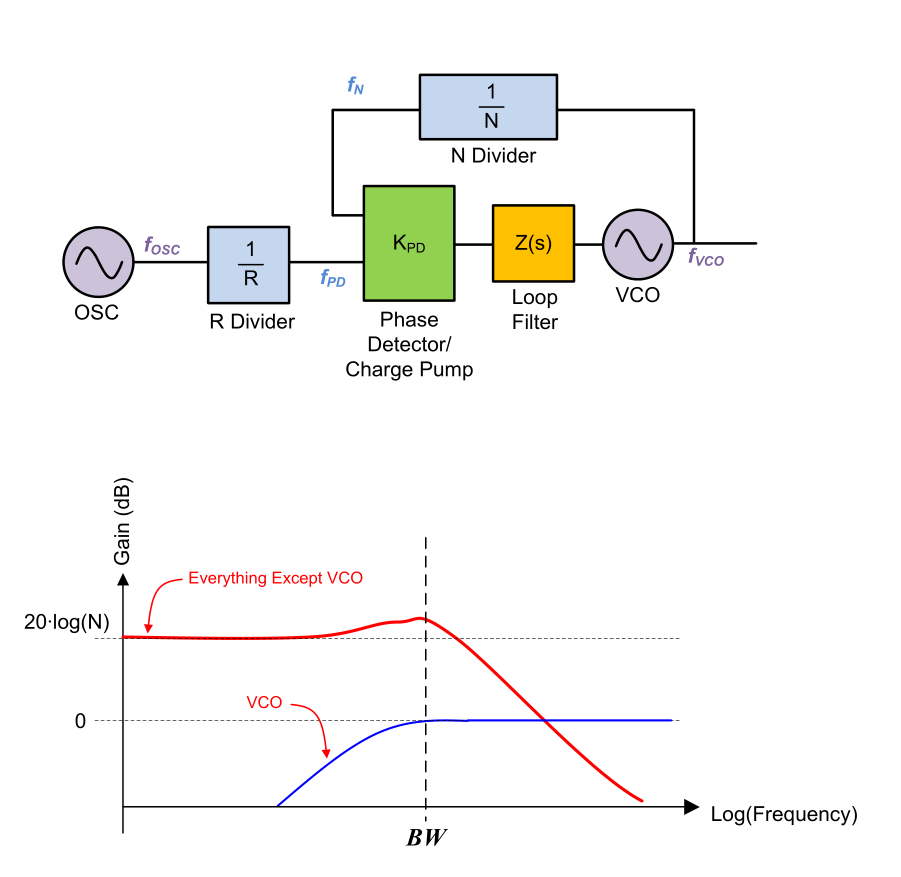
\includegraphics[width=\linewidth]{Figures/PLL_basics_regarding_VCO.png}
	\caption{Gain for VCO and  other blocks inside of PLL}
	\label{fig:PLL_basics_regarding_VCO	}
\end{figure}

\begin{info}
	For the VCO, the noise is suppressed below the loop bandwidth frequency and unshaped above the loop bandwidth.
\end{info}


% 50 or 100 ns for the SAW filter

% differential instead of pseudo differential 

% source degeneration


% \begin{question}[\itshape What kind of output is needed ?]
% 	s
% \end{question}


% Lorem ipsum dolor sit amet, consectetur adipiscing elit. Praesent porttitor arcu luctus, imperdiet urna iaculis, mattis eros. Pellentesque iaculis odio vel nisl ullamcorper, nec faucibus ipsum molestie. Sed dictum nisl non aliquet porttitor. Etiam vulputate arcu dignissim, finibus sem et, viverra nisl. Aenean luctus congue massa, ut laoreet metus ornare in. Nunc fermentum nisi imperdiet lectus tincidunt vestibulum at ac elit. Nulla mattis nisl eu malesuada suscipit.

% % Math equation/formula
% \begin{equation}
% 	I = \int_{a}^{b} f(x) \; \text{d}x.
% \end{equation}

% Aliquam arcu turpis, ultrices sed luctus ac, vehicula id metus. Morbi eu feugiat velit, et tempus augue. Proin ac mattis tortor. Donec tincidunt, ante rhoncus luctus semper, arcu lorem lobortis justo, nec convallis ante quam quis lectus. Aenean tincidunt sodales massa, et hendrerit tellus mattis ac. Sed non pretium nibh. Donec cursus maximus luctus. Vivamus lobortis eros et massa porta porttitor.

% \begin{info} % Information block
% 	This is an interesting piece of information, to which the reader should pay special attention. Fusce varius orci ac magna dapibus porttitor. In tempor leo a neque bibendum sollicitudin. Nulla pretium fermentum nisi, eget sodales magna facilisis eu. Praesent aliquet nulla ut bibendum lacinia. Donec vel mauris vulputate, commodo ligula ut, egestas orci. Suspendisse commodo odio sed hendrerit lobortis. Donec finibus eros erat, vel ornare enim mattis et.
% \end{info}

% %----------------------------------------------------------------------------------------
% %	PROBLEM 1
% %----------------------------------------------------------------------------------------

% \section{Problem title} % Numbered section

% In hac habitasse platea dictumst. Curabitur mattis elit sit amet justo luctus vestibulum. In hac habitasse platea dictumst. Pellentesque lobortis justo enim, a condimentum massa tempor eu. Ut quis nulla a quam pretium eleifend nec eu nisl. Nam cursus porttitor eros, sed luctus ligula convallis quis. Nam convallis, ligula in auctor euismod, ligula mauris fringilla tellus, et egestas mauris odio eget diam. Praesent sodales in ipsum eu dictum.

% %------------------------------------------------

% \subsection{Theoretical viewpoint}

% Maecenas consectetur metus at tellus finibus condimentum. Proin arcu lectus, ultrices non tincidunt et, tincidunt ut quam. Integer luctus posuere est, non maximus ante dignissim quis. Nunc a cursus erat. Curabitur suscipit nibh in tincidunt sagittis. Nam malesuada vestibulum quam id gravida. Proin ut dapibus velit. Vestibulum eget quam quis ipsum semper convallis. Duis consectetur nibh ac diam dignissim, id condimentum enim dictum. Nam aliquet ligula eu magna pellentesque, nec sagittis leo lobortis. Aenean tincidunt dignissim egestas. Morbi efficitur risus ante, id tincidunt odio pulvinar vitae.

% Curabitur tempus hendrerit nulla. Donec faucibus lobortis nibh pharetra sagittis. Sed magna sem, posuere eget sem vitae, finibus consequat libero. Cras aliquet sagittis erat ut semper. Aenean vel enim ipsum. Fusce ut felis at eros sagittis bibendum mollis lobortis libero. Donec laoreet nisl vel risus lacinia elementum non nec lacus. Nullam luctus, nulla volutpat ultricies ultrices, quam massa placerat augue, ut fringilla urna lectus nec nibh. Vestibulum efficitur condimentum orci a semper. Pellentesque ut metus pretium lacus maximus semper. Sed tellus augue, consectetur rhoncus eleifend vel, imperdiet nec turpis. Nulla ligula ante, malesuada quis orci a, ultricies blandit elit.

% % Numbered question, with subquestions in an enumerate environment
% \begin{question}
% 	Quisque ullamcorper placerat ipsum. Cras nibh. Morbi vel justo vitae lacus tincidunt ultrices. Lorem ipsum dolor sit amet, consectetuer adipiscing elit.

% 	% Subquestions numbered with letters
% 	\begin{enumerate}[(a)]
% 		\item Do this.
% 		\item Do that.
% 		\item Do something else.
% 	\end{enumerate}
% \end{question}
	
% %------------------------------------------------

% \subsection{Algorithmic issues}

% In malesuada ullamcorper urna, sed dapibus diam sollicitudin non. Donec elit odio, accumsan ac nisl a, tempor imperdiet eros. Donec porta tortor eu risus consequat, a pharetra tortor tristique. Morbi sit amet laoreet erat. Morbi et luctus diam, quis porta ipsum. Quisque libero dolor, suscipit id facilisis eget, sodales volutpat dolor. Nullam vulputate interdum aliquam. Mauris id convallis erat, ut vehicula neque. Sed auctor nibh et elit fringilla, nec ultricies dui sollicitudin. Vestibulum vestibulum luctus metus venenatis facilisis. Suspendisse iaculis augue at vehicula ornare. Sed vel eros ut velit fermentum porttitor sed sed massa. Fusce venenatis, metus a rutrum sagittis, enim ex maximus velit, id semper nisi velit eu purus.

% \begin{center}
% 	\begin{minipage}{0.5\linewidth} % Adjust the minipage width to accomodate for the length of algorithm lines
% 		\begin{algorithm}[H]
% 			\KwIn{$(a, b)$, two floating-point numbers}  % Algorithm inputs
% 			\KwResult{$(c, d)$, such that $a+b = c + d$} % Algorithm outputs/results
% 			\medskip
% 			\If{$\vert b\vert > \vert a\vert$}{
% 				exchange $a$ and $b$ \;
% 			}
% 			$c \leftarrow a + b$ \;
% 			$z \leftarrow c - a$ \;
% 			$d \leftarrow b - z$ \;
% 			{\bf return} $(c,d)$ \;
% 			\caption{\texttt{FastTwoSum}} % Algorithm name
% 			\label{alg:fastTwoSum}   % optional label to refer to
% 		\end{algorithm}
% 	\end{minipage}
% \end{center}

% Fusce varius orci ac magna dapibus porttitor. In tempor leo a neque bibendum sollicitudin. Nulla pretium fermentum nisi, eget sodales magna facilisis eu. Praesent aliquet nulla ut bibendum lacinia. Donec vel mauris vulputate, commodo ligula ut, egestas orci. Suspendisse commodo odio sed hendrerit lobortis. Donec finibus eros erat, vel ornare enim mattis et.

% % Numbered question, with an optional title
% \begin{question}[\itshape (with optional title)]
% 	In congue risus leo, in gravida enim viverra id. Donec eros mauris, bibendum vel dui at, tempor commodo augue. In vel lobortis lacus. Nam ornare ullamcorper mauris vel molestie. Maecenas vehicula ornare turpis, vitae fringilla orci consectetur vel. Nam pulvinar justo nec neque egestas tristique. Donec ac dolor at libero congue varius sed vitae lectus. Donec et tristique nulla, sit amet scelerisque orci. Maecenas a vestibulum lectus, vitae gravida nulla. Proin eget volutpat orci. Morbi eu aliquet turpis. Vivamus molestie urna quis tempor tristique. Proin hendrerit sem nec tempor sollicitudin.
% \end{question}

% Mauris interdum porttitor fringilla. Proin tincidunt sodales leo at ornare. Donec tempus magna non mauris gravida luctus. Cras vitae arcu vitae mauris eleifend scelerisque. Nam sem sapien, vulputate nec felis eu, blandit convallis risus. Pellentesque sollicitudin venenatis tincidunt. In et ipsum libero. Nullam tempor ligula a massa convallis pellentesque.

% %----------------------------------------------------------------------------------------
% %	PROBLEM 2
% %----------------------------------------------------------------------------------------

% \section{Implementation}

% Proin lobortis efficitur dictum. Pellentesque vitae pharetra eros, quis dignissim magna. Sed tellus leo, semper non vestibulum vel, tincidunt eu mi. Aenean pretium ut velit sed facilisis. Ut placerat urna facilisis dolor suscipit vehicula. Ut ut auctor nunc. Nulla non massa eros. Proin rhoncus arcu odio, eu lobortis metus sollicitudin eu. Duis maximus ex dui, id bibendum diam dignissim id. Aliquam quis lorem lorem. Phasellus sagittis aliquet dolor, vulputate cursus dolor convallis vel. Suspendisse eu tellus feugiat, bibendum lectus quis, fermentum nunc. Nunc euismod condimentum magna nec bibendum. Curabitur elementum nibh eu sem cursus, eu aliquam leo rutrum. Sed bibendum augue sit amet pharetra ullamcorper. Aenean congue sit amet tortor vitae feugiat.

% In congue risus leo, in gravida enim viverra id. Donec eros mauris, bibendum vel dui at, tempor commodo augue. In vel lobortis lacus. Nam ornare ullamcorper mauris vel molestie. Maecenas vehicula ornare turpis, vitae fringilla orci consectetur vel. Nam pulvinar justo nec neque egestas tristique. Donec ac dolor at libero congue varius sed vitae lectus. Donec et tristique nulla, sit amet scelerisque orci. Maecenas a vestibulum lectus, vitae gravida nulla. Proin eget volutpat orci. Morbi eu aliquet turpis. Vivamus molestie urna quis tempor tristique. Proin hendrerit sem nec tempor sollicitudin.

% % File contents
% \begin{file}[hello.py]
% \begin{lstlisting}[language=Python]
% #! /usr/bin/python

% import sys
% sys.stdout.write("Hello World!\n")
% \end{lstlisting}
% \end{file}

% Fusce eleifend porttitor arcu, id accumsan elit pharetra eget. Mauris luctus velit sit amet est sodales rhoncus. Donec cursus suscipit justo, sed tristique ipsum fermentum nec. Ut tortor ex, ullamcorper varius congue in, efficitur a tellus. Vivamus ut rutrum nisi. Phasellus sit amet enim efficitur, aliquam nulla id, lacinia mauris. Quisque viverra libero ac magna maximus efficitur. Interdum et malesuada fames ac ante ipsum primis in faucibus. Vestibulum mollis eros in tellus fermentum, vitae tristique justo finibus. Sed quis vehicula nibh. Etiam nulla justo, pellentesque id sapien at, semper aliquam arcu. Integer at commodo arcu. Quisque dapibus ut lacus eget vulputate.

% % Command-line "screenshot"
% \begin{commandline}
% 	\begin{verbatim}
% 		$ chmod +x hello.py
% 		$ ./hello.py

% 		Hello World!
% 	\end{verbatim}
% \end{commandline}

% Vestibulum sodales orci a nisi interdum tristique. In dictum vehicula dui, eget bibendum purus elementum eu. Pellentesque lobortis mattis mauris, non feugiat dolor vulputate a. Cras porttitor dapibus lacus at pulvinar. Praesent eu nunc et libero porttitor malesuada tempus quis massa. Aenean cursus ipsum a velit ultricies sagittis. Sed non leo ullamcorper, suscipit massa ut, pulvinar erat. Aliquam erat volutpat. Nulla non lacus vitae mi placerat tincidunt et ac diam. Aliquam tincidunt augue sem, ut vestibulum est volutpat eget. Suspendisse potenti. Integer condimentum, risus nec maximus elementum, lacus purus porta arcu, at ultrices diam nisl eget urna. Curabitur sollicitudin diam quis sollicitudin varius. Ut porta erat ornare laoreet euismod. In tincidunt purus dui, nec egestas dui convallis non. In vestibulum ipsum in dictum scelerisque.

% % Warning text, with a custom title
% \begin{warn}[Notice:]
%   In congue risus leo, in gravida enim viverra id. Donec eros mauris, bibendum vel dui at, tempor commodo augue. In vel lobortis lacus. Nam ornare ullamcorper mauris vel molestie. Maecenas vehicula ornare turpis, vitae fringilla orci consectetur vel. Nam pulvinar justo nec neque egestas tristique. Donec ac dolor at libero congue varius sed vitae lectus. Donec et tristique nulla, sit amet scelerisque orci. Maecenas a vestibulum lectus, vitae gravida nulla. Proin eget volutpat orci. Morbi eu aliquet turpis. Vivamus molestie urna quis tempor tristique. Proin hendrerit sem nec tempor sollicitudin.
% \end{warn}

% %----------------------------------------------------------------------------------------

\end{document}
